% Use only LaTeX2e, calling the article.cls class and 12-point type.

\documentclass[11pt]{article}

\usepackage[round,semicolon]{natbib}
\usepackage{etoolbox}
\AtBeginEnvironment{quote}{\singlespacing\tiny}
% Use times if you have the font installed; otherwise, comment out the
% following line.

% added by SKH
%\usepackage{lineno}
%\linenumbers

\usepackage{times}
\usepackage{amssymb}
\usepackage{amsmath}

\usepackage[export]{adjustbox}

\usepackage{graphicx}
\graphicspath{ {images/} }

% for adjustwidth
\usepackage{changepage}

% The following parameters seem to provide a reasonable page setup.

\topmargin 0.0cm
\oddsidemargin 1cm
\textwidth 15cm 
\textheight 21cm
\footskip 1.0cm

\usepackage{newfloat}
\usepackage{amsmath}
\usepackage[labelfont=bf]{caption}
\usepackage{nameref}
\usepackage{rotating}
\usepackage{color}
\usepackage{float}
\renewcommand{\figurename}{{}}
\renewcommand{\thefigure}{{Figure~\arabic{figure}}}

\renewcommand{\tablename}{{}}
\renewcommand{\thetable}{{Table~\arabic{table}}}

\newfloat{suppfile}{thp}{losuppfile}
\renewcommand{\thesuppfile}{Supplementary~file~\arabic{suppfile}}
\floatname{suppfile}{}

\newfloat{suppfig}{thp}{losuppfig}
\renewcommand{\thesuppfig}{Supplementary~figure~\arabic{suppfig}}
\floatname{suppfig}{}

%
\newfloat{supptable}{thp}{losupptable}
\renewcommand{\thesupptable}{Supplementary~table~\arabic{supptable}}
\floatname{supptable}{}
%

\renewcommand{\theequation}{Equation~\arabic{equation}}

\newcommand\skhcomment[1]{{\color{cyan}[#1]}}
\newcommand\jdbcomment[1]{{\color{red}[#1]}}


\usepackage{hyperref}
\hypersetup{colorlinks,citecolor=blue,linkcolor=blue,urlcolor=blue}
\hypersetup{colorlinks,citecolor=blue,linkcolor=blue,urlcolor=blue}

\usepackage{seqsplit}

\usepackage{array}
\newcolumntype{P}[1]{>{\raggedright\arraybackslash}p{#1}}

\title{Modeling site-specific amino-acid preferences deepens phylogenetic estimates of the divergence of viral proteins.} 

\author
{Sarah K. Hilton$^{1,2}$  and Jesse D. Bloom$^{1,2}$\\
\\
\normalsize{$^1$Division of Basic Sciences and Computational Biology Program,}\\
\normalsize{Fred Hutchinson Cancer Research Center, Seattle, WA 98109, USA}\\
\normalsize{$^2$Department of Genome Sciences, University of Washington, Seattle, WA}\\
\normalsize{E-mail:  jbloom@fredhutch.org.}\\
}


% Include the date command, but leave its argument blank.

\date{}

\usepackage{setspace}
\onehalfspacing


\begin{document} 

% Make the title.

\maketitle 


\begin{abstract}
\noindent  
Molecular phylogenetics can be used to estimate the time since the divergence of modern gene sequences.
For highly diverged sequences, such phylogenetic techniques often estimate surprisingly recent divergence times. 
In the case of viruses, there is independent evidence that the estimates of deep divergence times from molecular phylogenetics are too recent.
This discrepancy is caused in part by inadequate models of purifying selection leading to branch-length underestimation.
Here we show that models which account for purifying selection through experimental measurements of site-specific amino-acid preferences lengthen deep branches on phylogenies of influenza virus hemagglutinin.
This deepening of branch lengths is due to more realistic stationary states of the models, and is independent of the branch-length-extension from modeling site-to-site variation in amino-acid substitution rate.
The branch-length extension from experimentally informed site-specific models is similar to that achieved by other approaches that allow the stationary state to vary across sites.
However, the improvements from these site-specific but time-homogeneous and site-independent models are limited by the fact that a protein's amino-acid preferences gradually shift as it evolves.
Overall, our work underscores the importance of modeling how site-specific purifying selection affects the stationary state when estimating deep divergence times---but also shows the inherent limitations of approaches that fail to model how this selection shifts over time. 
\end{abstract}

\clearpage

\section*{Introduction} 

When studying a protein's evolutionary history, it is important to understand the timescale at which the evolutionary events have occurred. 
For example, understanding how long a particular viral lineage has been circulating informs hypotheses about population size, evolutionary rate, and possible previous hosts. Molecular phylogenetic is commonly used to make sure estimates of time since the divergence of two lineages. 
Under a molecular clock assumption, the branch lengths on a phylogenetic tree can be transformed into estimates of absolute time. 
However, it has been observed that these phylogenetic estimates often appear to estimate times since deep divergences that appear to be too recent. 
That is, when two nodes are separated by a very long branch, the phylogenetic estimate of this branch length often appears to be too short, which leads to an estimate of time that is too recent. 

In the case of viruses, there is independent evidence that the estimates of these deep divergences are indeed too recent. 
The times since the divergence of lineages within lentiviruses, paramyxoviruses and filoviruses have been estimated by methods which rely on information outside of or in addition to the viral phylogenetic tree.  
These independent estimates are often orders of magnitude older than the estimates using the viral phylogenetic tree only. 
For example, there are multiple examples of filovirus integrations into the genomes of rodents. 
Using these viral integrations and the fossil dates of the rodent species tree, the divergence of two main filovirus groups has been estimated to be $>7$ millions years ago. 
This estimate stands in stark contrast to the phylogenetic estimate of filovirus divergence which estimates this event happened $\sim 10,000$ years ago. 
All together, this indicates that phylogenetic branch length estimation does truly have a systematic bias towards underestimation. 

Branch length underestimation is due in part to inadequate modeling of purifying selection. 
During evolution, protein sites do not sample all 20 available amino-acids equally. 
Instead, proteins have site-specific amino-acid preferences which are necessary to maintain the structure and function of the protein. 
Failure to account for these constraints will lead to branch length underestimation because the model will assume that sequences which have been evolving for a very long period of time should be more diverged than is actually the case. 
Furthermore, the site-specific amino-acid preferences at one site are often dependent on the amino-acid identity at another site. 
As a result, the preferences ``shift" over time time due to the accumulation of substitutions in other parts of the protein.  

Most phylogenetic substitution models are time-homogenous and site-independent: they do not take into account how sites may interact with each other or how preferences may shift over time. 
However, they can model purifying selection with varying degrees of complexity. 
One method is to allow the parameter controlling the rate of nonsynonymous to synonymous substitution, the dN/dS parameter, to vary among the protein sites. 
This variation accounts for the fact that constrained sites will have a lower rate of amino-acid substitution than mutationally constrained sites. 
However, the stationary state of this model, which describes the expected sequence composition after a very long evolutionary time, will be exactly the same as a model without any variation in the dN/dS parameter. 
Alternatively, models can have site-specific stationary states which explicitly acknowledge the protein's site-specific amino-acid preferences. 
Such models should estimate deep divergence times because model still expects relatively low sequence divergence even after a very long evolutionary time. 

Here, we tested the effect of modeling site-specific amino-acid preferences though a model with a site-specific stationary state on an influenza hemagglutinin (HA) phylogenetic tree. 
Specifically, we used Experimentally Informed Codon Models (ExpCM's) defined by site-specific amino-acid preferences measured by a high-throughput functional assay called deep mutational scanning. 
We found that these ExpCM's estimated longer branches. 
We found that the extension in branch length due modeling purifying selection via a site-specific stationary state is largely independent of the the effect of modeling purifying selection through rate variation. 
However, our results make it clear that the site-specific amino-preferences of HA are constant across the entire tree. 
In particular, the branch lengthening is most pronounced near the sequence of the HA that was used in the deep mutational scanning experiment that parameterized the ExpCM.
These results underscore the importance of modeling how site-specific purifying selection affects the stationary state when estimating deep divergence times---but also shows the inherent limitations of approaches that fail to model how this selection shifts over time. 


\section*{Results}

\subsection*{Different ways substitution models account for purifying selection}

\begin{figure}
\centerline{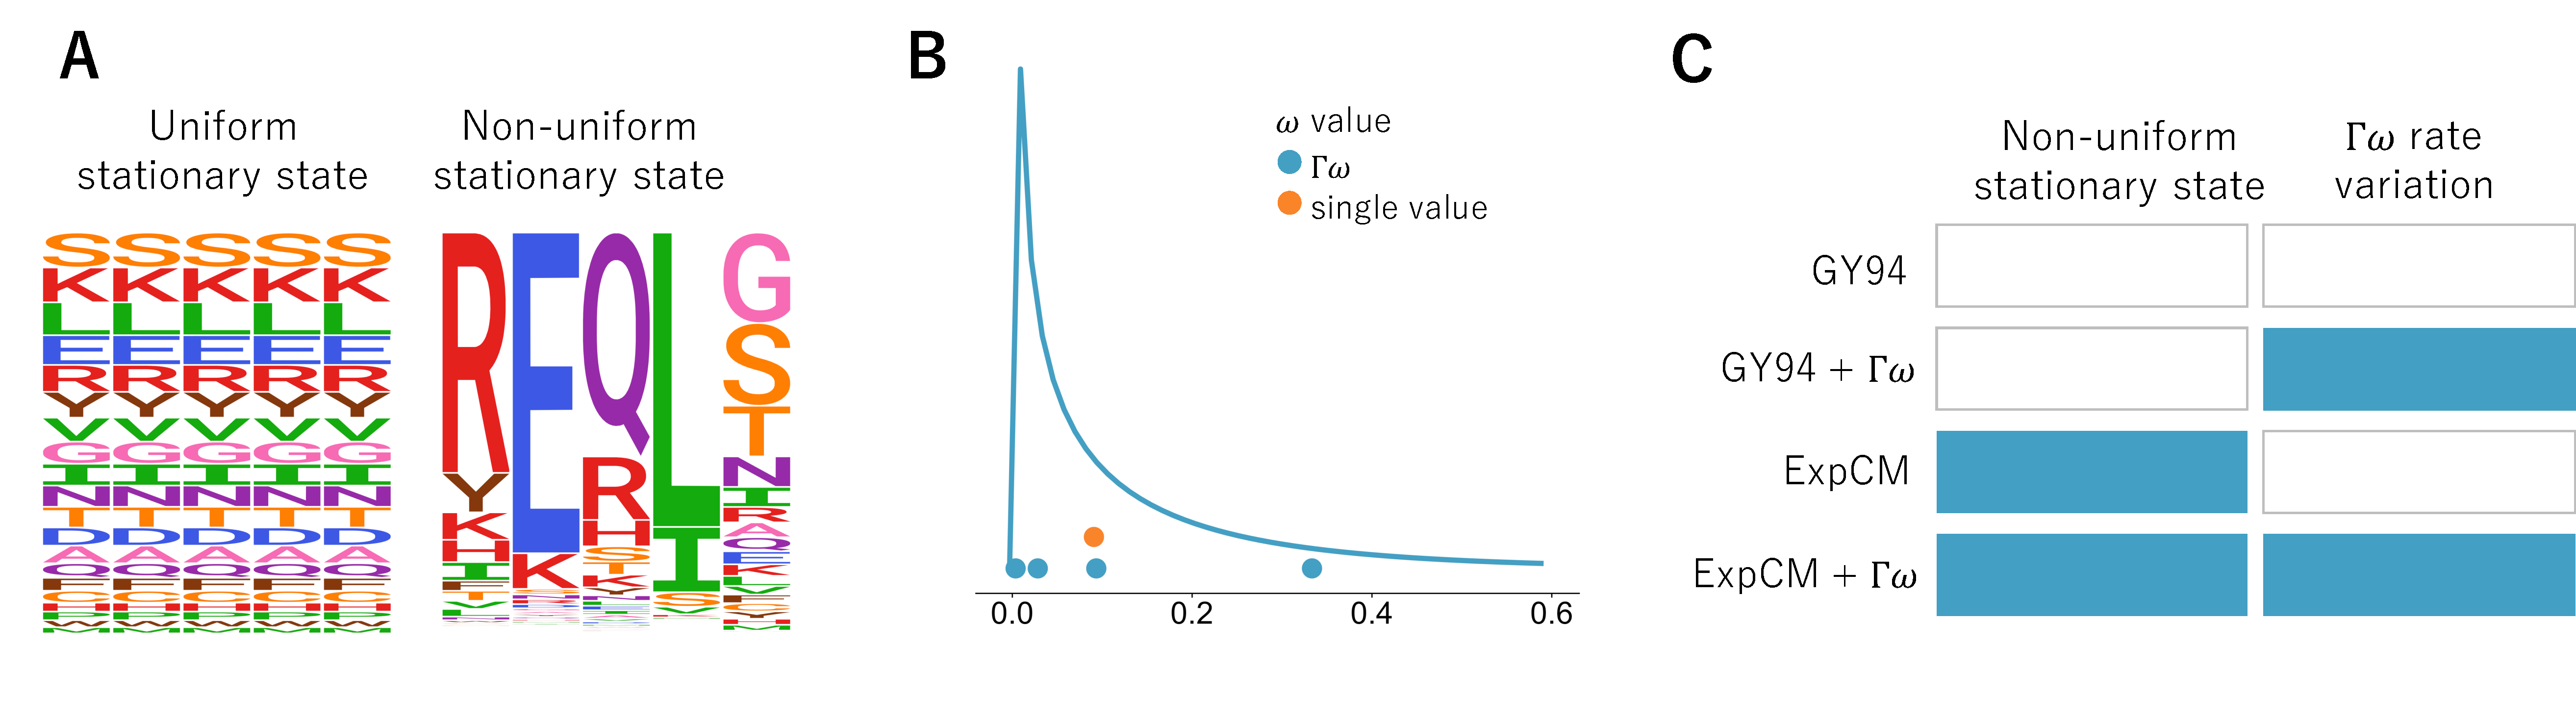
\includegraphics[width=0.90\textwidth]{figures/model_feature.pdf}}
\caption{\label{fig:model_feature}
\textbf{Different ways codon models account for purifying selection.}
(A) The dN/dS parameter, $\omega$, can be defined as one gene-wide average (orange triangle) or allowed to vary according to some statistical distribution (blue circles). 
For computational tractability, the distribution is discretized into $K$ bins and $\omega$ takes on the mean of each bin~\citep{yang1994maximum,yang2000codon}. 
A gamma distribution ($\Gamma$) with $K=4$ bins is shown here.
(B) A substitution model's stationary state defines the expected sequence composition after a very long evolutionary time. 
Most substitution models have stationary states that are uniform across sites.
However, substitution models can have site-specific stationary states.
In the logo plots, each column is a site in the protein and the height of each letter is the frequency of that amino acid at stationary state. 
(C) Substitution models can incorporate neither, one, or both of these features.
Here we will use substitution models from the Goldman-Yang~\citep[GY94;][]{goldman1994codon,yang2000codon} and experimentally informed codon model~\citep[ExpCM;][]{hilton2017phydms} families with and without gamma-distributed $\omega$ to represent all possible combinations.
}
\end{figure}

Proteins evolve under purifying selection to maintain their structure and function. 
This purifying selection is not homogenous across sites in a protein.
It is also not homogenous among the different amino acids at a given site.
For instance, some protein sites strongly prefer hydrophobic amino acids, others are constrained to just one or a few amino acids, and yet others tolerate many amino acids.
In general, these constraints are highly idiosyncratic among sites, and so pose a challenge for phylogenetic substitution models.

Here we consider how purifying selection is handled by codon models, which are the most accurate of the three classes (nucleotide, amino acid, and nucleotide) of phylogenetic substitution models in widespread use~\citep{arenas2015trends}.
Standard codon models distinguish between two types of substitutions: synonymous and nonsynonymous.
The relative rate of these substitutions is referred to as dN/dS or $\omega$.
In their simplest form, codon substitution models fit a single $\omega$ that represents the gene-wide average fixation rate of nonsynonymous mutations relative to synonymous ones.
Here we will use such substitution models in the form proposed by \citet{goldman1994codon}.
When these models have a single gene-wide $\omega$ they are classified as M0 by \citet{yang2000codon}.
Here we will refer to M0 Goldman-Yang models simply as GY94 models (\ref{eq:GY94}). 
The gene-wide $\omega$ is usually $<1$~\citep{murrell2015gene}, and crudely represents the fact that many amino-acid substitutions are under purifying selection.

A single gene-wide $\omega$ ignores the fact that purifying selection is heterogeneous across sites.
The most common strategy to ameliorate this defect is to allow $\omega$ to vary among sites according to some statistical distribution~\citep{yang1994maximum,yang2000codon}.
For instance, in the M5 variant of the GY94 model~\citep{yang2000codon}, $\omega$ follows a gamma distribution as shown in \ref{fig:model_feature}A.
We will denote this model as GY94+$\Gamma\omega$.
A GY94+$\Gamma\omega$ captures the fact that the rate of nonsynonymous substitution can vary across sites. 
However, this formulation treats all nonsynonymous substitutions equivalently, since the rate is agnostic to the amino-acid identity of the mutation. 

A model formulation that accounts for the fact that purifying selection depends on the specific amino-acid mutation is provided by so-called ``mutation-selection'' models~\citep{halpern1998evolutionary,yang2008mutation,rodrigue2010mutation,tamuri2012estimating,mccandlish2014modeling}.
These models explicitly define a different set of amino-acid preferences at each site in the protein. 
This more mechanistic formulation results in a site-specific stationary state (\ref{fig:model_feature}B). 
These models capture the site-to-site variation in amino-acid composition that is an obvious features of real proteins, and usually better describe actual evolution than models with only rate variation~\citep{lartillot2004bayesian, le2008phylogenetic, rodrigue2010mutation,hilton2017phydms,bloom2014experimentally}.

However, the increased realism of mutation-selection models comes at the cost of an increased number of parameters. 
Codon substitution models with uniform stationary states have only a modest number of parameters that must be fit from the phylogenetic data.
For instance, a GY94+$\Gamma\omega$ model with the commonly used F3X4 stationary state has 12 parameters: two describing the shape of the gamma distribution over $\omega$, a transition-transversion rate, and nine parameters describing the nucleotide composition of the stationary state.
However, mutation-selection models must additionally specify 19 parameters defining the stationary state for \emph{each} site (there are 20 amino acids whose frequencies are constrained to sum to one).
This corresponds to $19\times L$ parameters for a protein of length $L$, or 9,500 parameters for a 500-residue protein.
It is challenging to obtain values for these parameters in a maximum-likelihood framework without overfitting the data~\citep{rodrigue2013statistical}.
\skhcomment{Do we need to comment on the tamuri paper?}
Here we will primarily use experimentally informed codon models~\citep[ExpCM's, \ref{eq:ExpCM};][]{bloom2014experimentally, hilton2017phydms, bloom2017identification} which define these parameters \textit{a priori} from deep mutational scanning experiments so they do not need to be fit from phylogenetic data.
The number of remaining free parameters for an ExpCM is similar to a non-site-specific substitution model.
An alternative strategy of obtaining parameters for site-specific stationary states via Bayesian inference~\citep{lartillot2004bayesian, rodrigue2014site} is discussed in the last section of the Results.

Importantly, these two strategies for modeling purifying selection are not mutually exclusive.
Mutation-selection models such as ExpCM can still incorporate an $\omega$ parameter~\citep{rodrigue2016detecting, bloom2017identification}, which now represents the relative rate of nonsynonymous to synonymous substitution \emph{after} accounting for the constraints due to the site-specific stationary state.
This $\omega$ parameter for an ExpCM can be drawn from a distribution just like for GY94-style models~\citep{haddox2017mapping, rodrigue2014site}. 
We will denote such models as ExpCM+$\Gamma\omega$.
\ref{fig:model_feature}C shows the full spectrum of models that incorporate all combinations of gamma-distributed $\omega$ and site-specific stationary states.

\subsection*{Effect of stationary state and rate variation on branch-length estimation}

\begin{figure}
\centerline{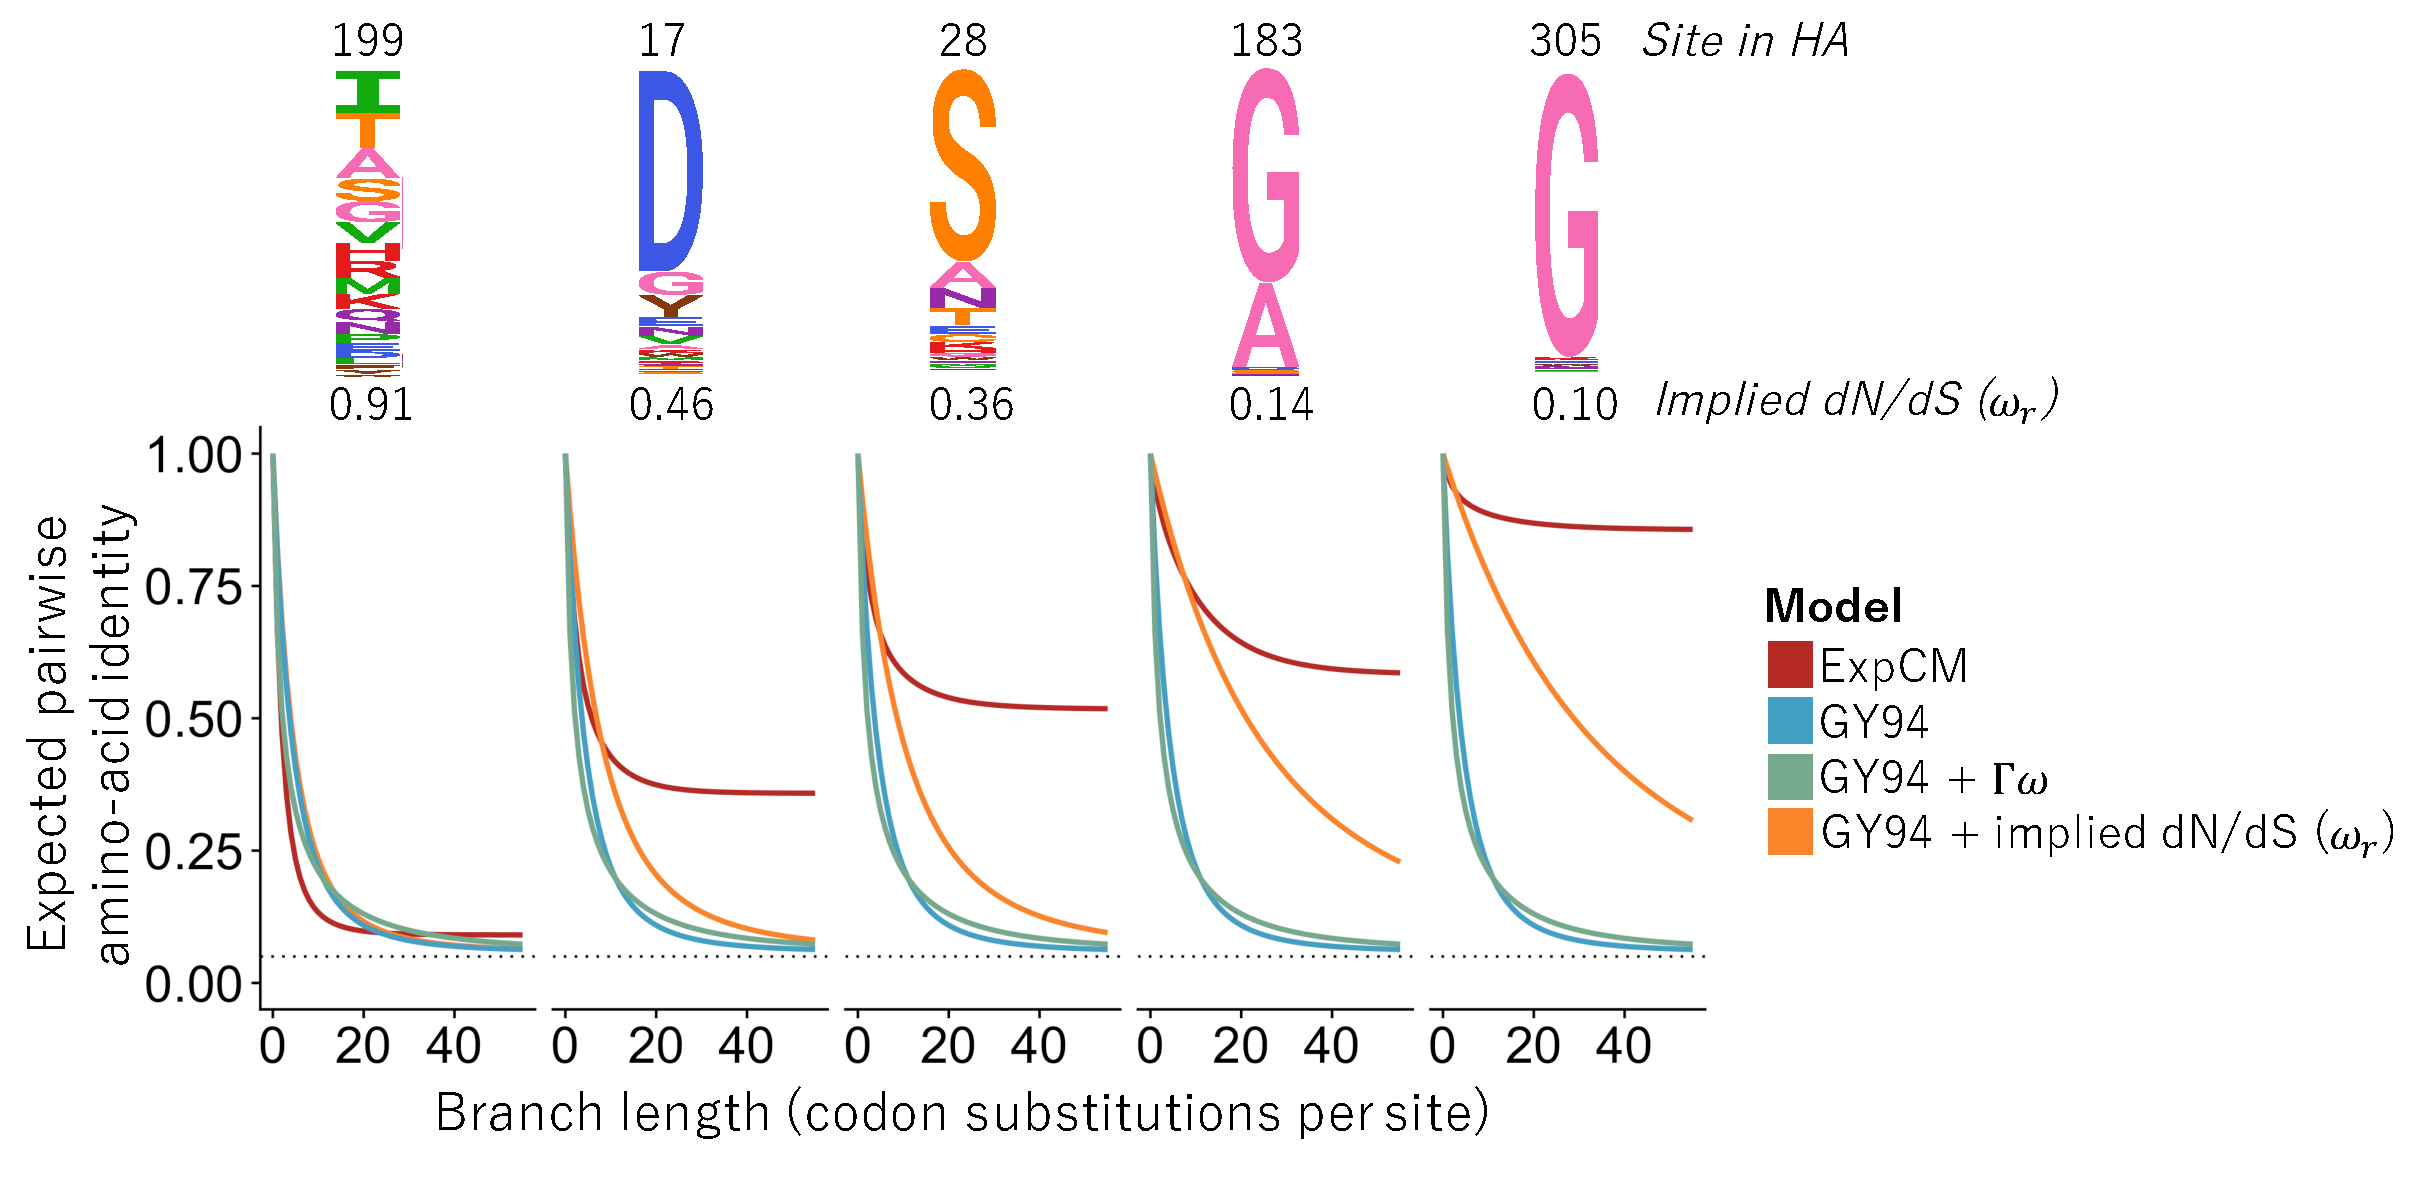
\includegraphics[width=0.90\textwidth]{figures/decay.pdf}}
\caption{\label{fig:decay}
\textbf{Effect of stationary state and $\Gamma\omega$ rate variation on predicted asymptotic sequence divergence.}
The logo plots at top show the amino-acid preferences for some sites in an H1 influenza hemagglutinin protein as experimentally measured by~\citet{doud2016accurate}.
The graphs show the expected amino-acid identity at that site for two sequences separated by a branch of the indicated length (\ref{eq:f}).
For the GY94 model, the graphs are identical for all sites since this model does not have site-specific parameters; the same is true for GY94+$\Gamma\omega$.
The graphs do differ among sites if we use the amino-acid preferences to calculate a different $\omega_r$ value for each site $r$ in a GY94 framework~\citep[\ref{eq:w_r};][]{spielman2015relationship}.
However, all GY94 models, including the one with site-specific $\omega_r$ values, approach the same asymptote since they all have the same stationary state.
But the ExpCM has different asymptotes for different sites since it accounts for how amino-acid preferences lead to site-specific stationary states.
}
\end{figure}

Given a single branch, a substitution model transforms sequence identity into branch length.
Under a molecular-clock assumption, this branch length is proportional to time.
The transformation from sequence identity to branch length is trivial when the sequence identity is high.
For instance, when there has only been one substitution, then the sequence identity will simply be $\frac{L - 1}{L}$ for a gene of $L$ sites, and even a simple exponential model~\citep{zuckerkandl1965} will correctly infer the short branch length of $1/L$ substitutions per site.
However, as substitutions accumulate it becomes progressively more likely for multiple changes to occur at the same site.
In this regime, the accuracy of the substitution model becomes critical for transforming sequence identity into branch length.
Any time-homogenous substitution model predicts that after a very large number of substitutions, two related sequences will approach some amino-acid asymptotic sequence identity.
For instance, if all 20 amino acids are equally likely in the stationary state, then this asymptotic sequence identity will be 0.05.
If the substitution model underestimates the asymptotic sequence identity then it will also underestimate long branch lengths, since it will predict that sequences that have evolved for a very long time should be more diverged than is actually the case.

\ref{fig:decay} shows how different substitution models predict sequence identity to decrease as a function of branch length using model parameters fit to a phylogeny of H1 influenza hemagglutinin (HA) genes.
The GY94 model predicts the same behavior for all sites, since it does not have any site-specific parameters.
This model predicts an asymptotic sequence divergence of 0.059, which is slightly higher than 0.050 since some of the 20 amino acids are favored due to more redundant codons and biases towards certain nucleotides.
Intuitively, this asymptotic sequence identity of 0.059 seems low, since like many proteins HA has a highly conserved structure and function that imposes constraints that cause most sites to sample only a small subset of the 20 amino acids among all known HA homologs~\citep{nobusawa1991comparison}.

Accounting for site-to-site rate variation in GY94 models affects the rate at which the asymptotic sequence identity is approached, but not the actual value of this asymptote. 
For instance, \ref{fig:decay} shows that the GY94+$\Gamma\omega$ model takes longer to reach the asymptote than GY94, but the asymptote for both models is identical. 
This fact holds true even if we use experimental measurements of HA's site-specific amino-acid preferences~\citep{doud2016accurate} to calculate a different $\omega_r$ value for each site using the method of \citet{spielman2015relationship} (see \ref{eq:w_r}).
Specifically, this GY94+$\omega_r$ model predicts that different sites will approach the asymptote at different rates, but the asymptote is always the same (\ref{fig:decay}).
The invariance of the asymptotic sequence identity under different schemes for modeling $\omega$ is a fundamental feature of the mathematics of reversible substitution models.
These models are reversible stochastic matrices, which can be decomposed into stationary states and symmetric exchangeability matrices~\citep{nielsen2006statistical}.
The stationary state is invariant with respect to multiplication of the symmetric exchangeability matrix by any non-zero number.
Different schemes for modeling $\omega$ only multiply elements of the symmetric exchangeability matrix.
Therefore, no matter how ``well" a model accounts for site-to-site variation in $\omega$, it will always have the same stationary state as a simple GY94 model. 

However, mutation-selection models such as ExpCM's have site-specific stationary states.
Therefore, they predict that different sites will have different asymptotic sequence identities (\ref{fig:decay})---a prediction that accords with the empirical observation that some sites are much more variable than others in alignments of highly diverged sequences.
For instance, \ref{fig:decay} shows that at sites such as 348 and 305 in the H1 HA, an ExpCM but not a GY94-style model predicts that the divergence will always be low. 
When sites with highly constrained amino-acid preferences such as these are common, an ExpCM can estimate a long branch length at modest sequence identities that a GY94 model might attribute to a shorter branch.


\subsection*{Simulations demonstrate how failure to model site-specific stationary states leads to branch-length underestimation.}

\begin{figure}
\centerline{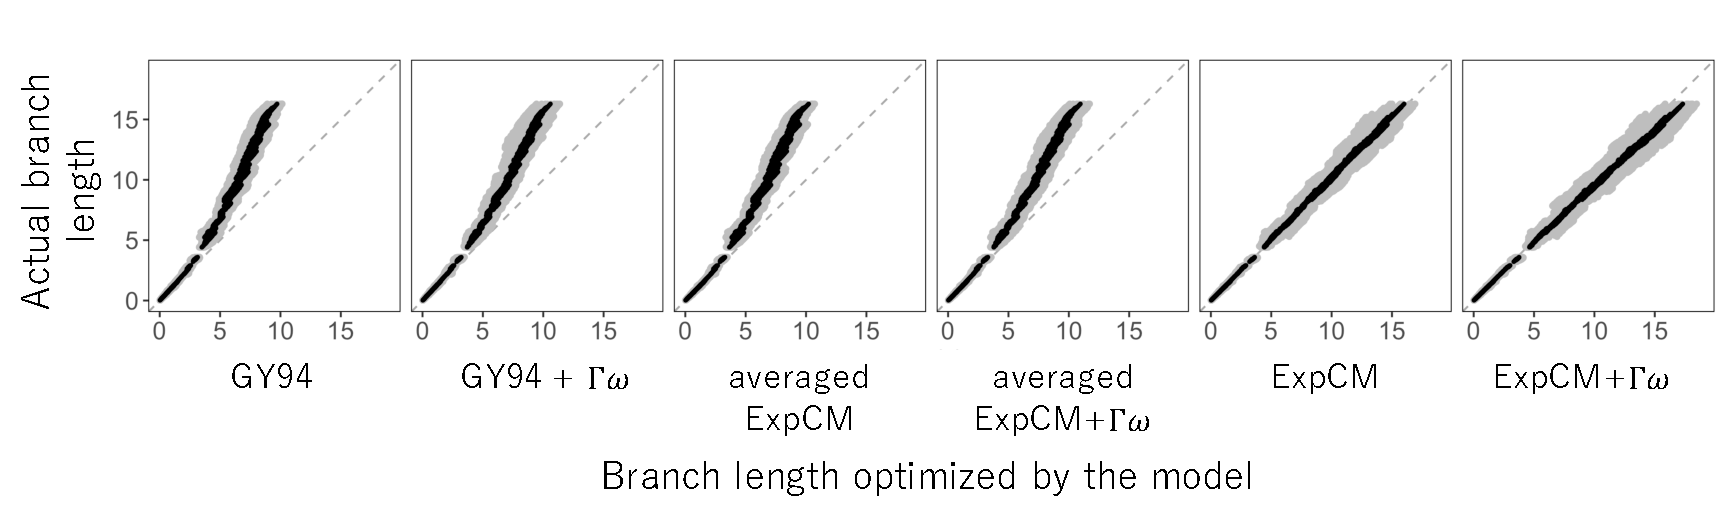
\includegraphics[width=0.85\textwidth]{figures/simulations}}
\caption{\label{fig:simulations}
\textbf{Branch lengths inferred on data simulated under a model with site-specific amino-acid preferences.} 
We simulated alignments along a phylogenetic tree of HA genes (see Figure~\ref{fig:empirical_trees}) using an ExpCM parameterized by the actual site-specific amino-acid preferences for an H1 HA~\citep{doud2016accurate}.
We then inferred the branch lengths of this tree on the simulated alignments.
The inferred branch lengths for various models are plotted on the x-axis, and the actual branch lengths used in the simulations are on the y-axis.
We performed 10 simulations and inferences, and gray points show each inferred branch length from each simulation, and black points show the average of each branch length across simulations.
The grey dashed line at $y=x$ represents the behavior of an unbiased estimator. 
}
\end{figure}

To directly demonstrate the effect of stationary state and $\Gamma\omega$ rate variation on branch-length estimation, we tested the ability of a variety of models to accurately infer branch lengths on simulated data (\ref{fig:simulations}).
Specifically, we simulated alignments of sequences along the HA phylogenetic tree in \ref{fig:empirical_trees} using an ExpCM parameterized by the amino-acid preferences of H1 HA as experimentally measured by deep mutational scanning~\citep{doud2016accurate}. We then estimated the branch lengths from the simulated sequences using all the substitution models in \ref{fig:model_feature}C, and compared these estimates to the actual branch lengths used in the simulations.

The models with a uniform stationary state underestimated the lengths of long branches on the phylogenetic tree of the simulated sequences (\ref{fig:simulations}). 
The GY94 model estimated branches lengths that are only about 60\% of the true values for the longest branches. 
Accounting for site-to-site variation in $\omega$ did not fix the fundamental problem: the GY94+$\Gamma\omega$ did slightly better, but still substantially underestimated the longest branches.
However, there was no systematic underestimation of long branches by the ExpCM and ExpCM+$\Gamma\omega$ models, which accurately accounted for the site-specific amino-acid preferences used in the simulations.
The improved performance of the ExpCM's is due to their site-specific modeling of the stationary state: if we parameterize these models by site-specific amino-acid preferences that have been averaged across HA sites, then they perform no better than GY94 models~\ref{fig:simulations}.
Therefore, models with uniform stationary states are fundamentally incapable of accurately estimating the length of long branches in phylogenies of sequences that have evolved under strong site-specific amino-acid preferences.


\subsection*{Experimentally informed site-specific models estimate longer branches on real data.}

\begin{figure}
\centerline{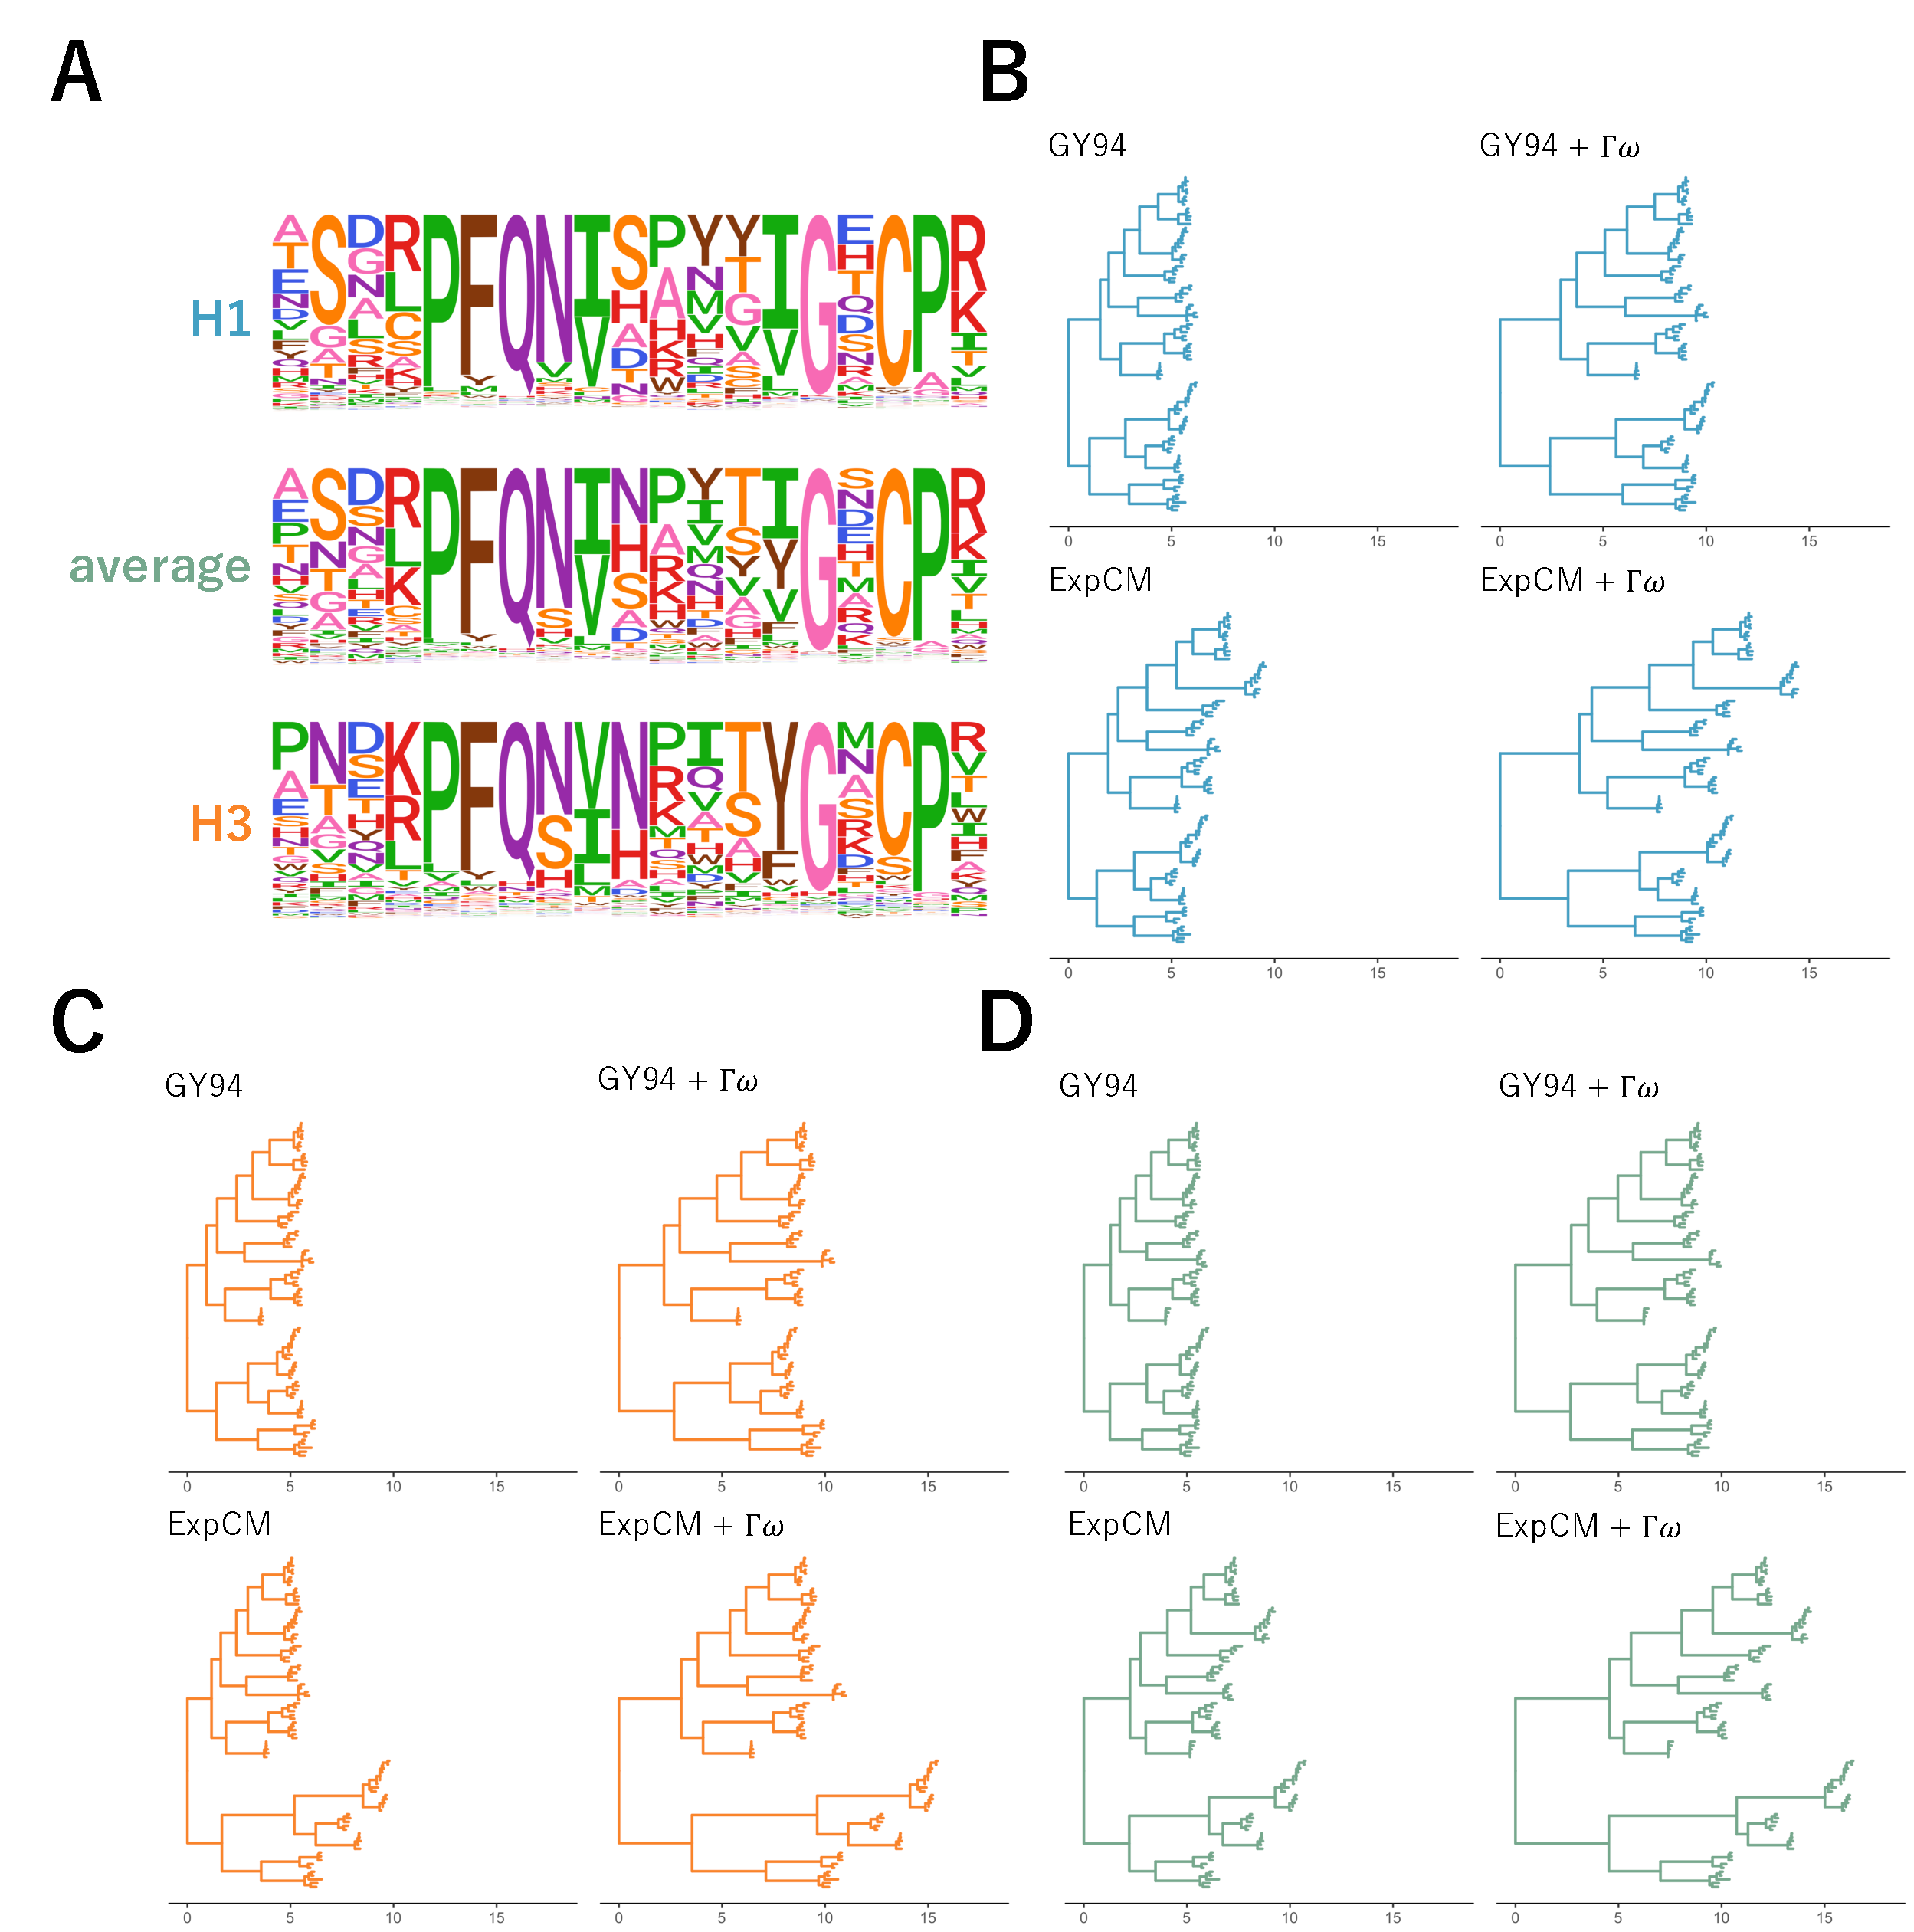
\includegraphics[width=\textwidth]{figures/empirical_trees.pdf}}
\caption{\label{fig:empirical_trees}
\textbf{Effect of site-specific stationary state and $\Gamma\omega$ rate variation on HA branch length estimation.} 
The branch lengths of the HA tree are optimized using the indicated ExpCM and GY94 models. 
The amino-acid preferences defining the model (ExpCM) or implied by the model (GY94) are shown as logoplots for 15 example sites in HA; the full set of experimentally measured amino-acid preferences defining each ExpCM are shown in \ref{suppfig:prefs_doud}, \ref{suppfig:prefs_lee}, and \ref{suppfig:prefs_average}. 
The ExpCM's use amino-acid preferences measured in deep mutational scanning of an H1 HA~\citep{doud2016accurate}, an H3 HA~\citep{lee2018deep}, or the average of the measurements for these two HAs.
The circle denotes the H1 clade and the triangle denotes the H3 clade. 
}
\end{figure}

\begin{table}[t!]
\caption{\label{tab:empirical_data}
{\bf Fitting of substitution models to the HA phylogenetic tree.}
The models fit here are the same ones in~\ref{fig:empirical_trees}. 
All ExpCMs describe the evolution of HA better than the GY94 models, as evaluated by the Akaike information criteria~\citep[$\Delta$AIC,][]{posada2004model}
The $\omega$ value for each of the $K=4$ bins is shown for the models with $\Gamma\omega$ rate variation. 
All ExpCM's fit a stringency parameter $>1$.
} 
     \begin{tabular}{cccccccccc}
        \hline
         Model & $\Delta$AIC & {\shortstack{Log\\ Likelihood}} & $\omega$ & {\shortstack{Stringency\\ parameter ($\beta$)}}\\ \hline
       	ExpCM  (H1+H3 avg) + $\Gamma\omega$  & 0 & -48751 & 0.19,  0.50,  0.90,  1.86 &  1.70\\
	ExpCM (H1+H3 avg)  &  950 & -49227 & 0.15 & 1.78\\
	ExpCM  (H1) + $\Gamma\omega$  & 1306 & -49404  & 0.13 ,  0.44,  0.91,  2.16 & 1.12\\
	ExpCM (H3) + $\Gamma\omega$ & 1737 & -49620 & 0.09,  0.33,  0.72,  1.77 & 1.28\\
	ExpCM (H1) & 2556 & -50030 &  0.13 & 1.22\\
	ExpCM (H3) &  3197 & -50350 & 0.12 & 1.45\\
	GY94 + $\Gamma\omega$  & 4719 & -51106 & 0.00,  0.03,  0.08,  0.26 & - \\
	GY94 & 7625 & -52560  & 0.07 & -\\
      \end{tabular}
\end{table}

The foregoing section shows the superiority of ExpCM's to GY94 models for estimating long branches on phylogenies simulated with ExpCM models.
But how do these models perform on real data?
Real genes do evolve under functional constraint, but these constraints are almost certainly more complex than what is modeled by an ExpCM.
However, if ExpCM's do a substantially better job than GY94 models of capturing the true constraints, then we might still expect them to estimate more accurate branch lengths.

To test the models on real data, we used actual sequences of influenza HA. 
The topology of HA phylogenetic trees (\ref{fig:empirical_trees}) makes these sequences an interesting test case for branch-length estimation.
HA consists of a number of different subtypes.
Sequences within a subtype have $>75\%$ amino-acid identity, but sequences in different subtypes have as little as 38\% identity.
However, HA proteins from all subtypes have a highly conserved structure that performs a highly conserved function~\citep{ha2002h5,russell2004h1}.
We used \texttt{RAxML}~\citep{stamatakis2006raxml} with a nucleotide substitution model  (GTRCAT) to infer a phylogenetic tree for 87 HA sequences drawn from 14 of the 18 subtypes (we excluded bat influenza and three other rare subtypes).
For the rest of this paper, we fix the tree topology to this \texttt{RAxML}-inferred tree.
Although the nucleotide model used with \texttt{RAxML} is probably less accurate than codon models, the modular subtype structure of the HA phylogeny means that most of the phylogenetic uncertainty lies in the length of the long branches separating the subtypes rather than in the tree topology itself.

There are two deep mutational scanning datasets for HA that estimated amino-acid preferences for all sites.
One scan measured the site-specific amino-acid preferences of an H1 HA~\citep{doud2016accurate} and the other measured the preferences of an H3 HA~\citep{lee2018deep}.
These two HAs have only $\sim$42\% amino-acid identity, and so are separated by a large distance on the phylogenetic tree (see triangle and circle on \ref{fig:empirical_trees}).
The experimentally measured amino-acid preferences clearly differ between the H1 and H3 HA at a substantial number of sites~\citep[][\ref{suppfig:prefs_doud}, 
\ref{suppfig:prefs_lee}]{lee2018deep}.
Therefore, we also created a third set of amino-acid preferences by averaging the preferences measured in the deep mutational scanning of the H1 and H3 HAs, under the conjecture that these averaged preferences might do a better job of describing the ``average'' constraint on sites across the full HA tree.
These three sets of HA amino-acid preferences define three different ExpCM's.
 
We fit the GY94 model and each of the three ExpCM's to the fixed HA tree topology estimated using \texttt{RAxML}, and also tested a version of each model with $\Gamma\omega$ rate variation.
\ref{tab:empirical_data} shows that all the ExpCM's fit the actual data much better than the GY94 models.
The best fit was for the ExpCM that was informed by the average of the H1 and H3 deep mutational scans.
For all models, incorporating $\Gamma\omega$ rate variation improved the fit, although even ExpCM's without $\Gamma\omega$ greatly outperformed the GY94+$\Gamma\omega$ models.
As mentioned in the previous section, $\omega$ generally takes on values $<1$ when fit to all sites in the gene~\citep{murrell2015gene}, and our results follow this trend. 
\ref{tab:empirical_data} shows that all models that fit a single $\omega$ fit very small values, reflecting strong purifying selection against amino-acid change in HA. 
However, the ExpCM's with a single $\omega$ always fit $\omega$ values greater than the GY94 model, suggesting that the site-specific stationary state of the ExpCM's captures some of the purifying selection that the GY94 models can represent only via a small omega.
Among the models with $\Gamma\omega$, the GY94 fits all four $\omega$ categories to values $<< 1$, but the ExpCM's all fit one of the four $\omega$ categories to a value $>1$.
This increase in $\omega$ values makes sense given the different interpretation of $\omega$ in each family of models. 
The ExpCM $\omega$ is the relative rate of fixation of nonsynonymous to synonymous mutations \textit{after} accounting for the functional constraints described by the deep mutational scanning amino-acid preferences.
This more realistic null model gives ExpCM's more power to detect diversifying selection~\citep{bloom2017identification, rodrigue2016detecting}, for amino-acid change, which occurs at some sites in HA due to immune selection.

Models which account for purifying selection via either $\Gamma\omega$ rate variation or a site-specific stationary state are not just better fit models, they also increase the estimation of branch length on the HA tree. 
As \ref{fig:empirical_trees} shows, the tree optimized by without $\Gamma\omega$ rate variation and without a site-specific stationary state, the GY94 model, estimated the shortest branches of all eight models. 
Specifically, the ExpCM's defined by H1 HA or H3 HA amino-acid preferences estimated a tree which overall length is $\sim 8\%$ longer than the GY94 tree and the GY94+$\Gamma\omega$ model estimated tree which is $\sim 36\%$ longer than the GY94 tree~\ref{supptab:tree_lengths}. 
But importantly, the effects from these two methods of modeling purifying selection are largely independent.
For every model (GY94 or any of the three ExpCM's), the $\Gamma\omega$ version estimates longer deep branches.
In addition, all ExpCM's estimate longer deep branches than the GY94 model, and all ExpCM+$\Gamma\omega$ models estimate longer deep branches than the GY94+$\Gamma\omega$ model.
\skhcomment{I think we can make a stronger statement about the independence of these effects. I did the calculation and 96\% of the branch length extension of GY94 vs. ExpCM(H1+H3)+$\Gamma\omega$ can be explained by simply adding the ``effect of adding $\Gamma\omega$" (GY94 vs. GY94+$\Gamma\omega$) and the ``effect of adding preferences" (GY94 vs. ExpCM(H1+H3). Do you think that is a useful analysis to include?}

However, while adding $\Gamma\omega$ rate variation increases the length of deep branches in a fashion that appears roughly uniform across the tree (\ref{fig:empirical_trees}), the branch lengthening from the ExpCM's is not uniform across the tree. 
In particular, the branch lengthening is most pronounced near the sequence of the HA that was used in the deep mutational scanning experiment that parameterized the ExpCM.
For instance, the ExpCM informed by the H1 data most dramatically lengthens branches near the H1 clade of the tree, while the ExpCM informed by the H3 data has the largest effect on branches near the H3 clade.
The ExpCM informed by the average of the H1 and H3 data has a more uniform effect, but still most strongly affects branches near either the H1 or H3 clades.
Therefore, \ref{fig:empirical_trees} shows that the ExpCM's estimate longer branches, but that the effect is biased by the set of preferences used to define the stationary state of the model.

\subsection*{Competing effects of shifting preferences and long branches.}

\begin{figure}
\centerline{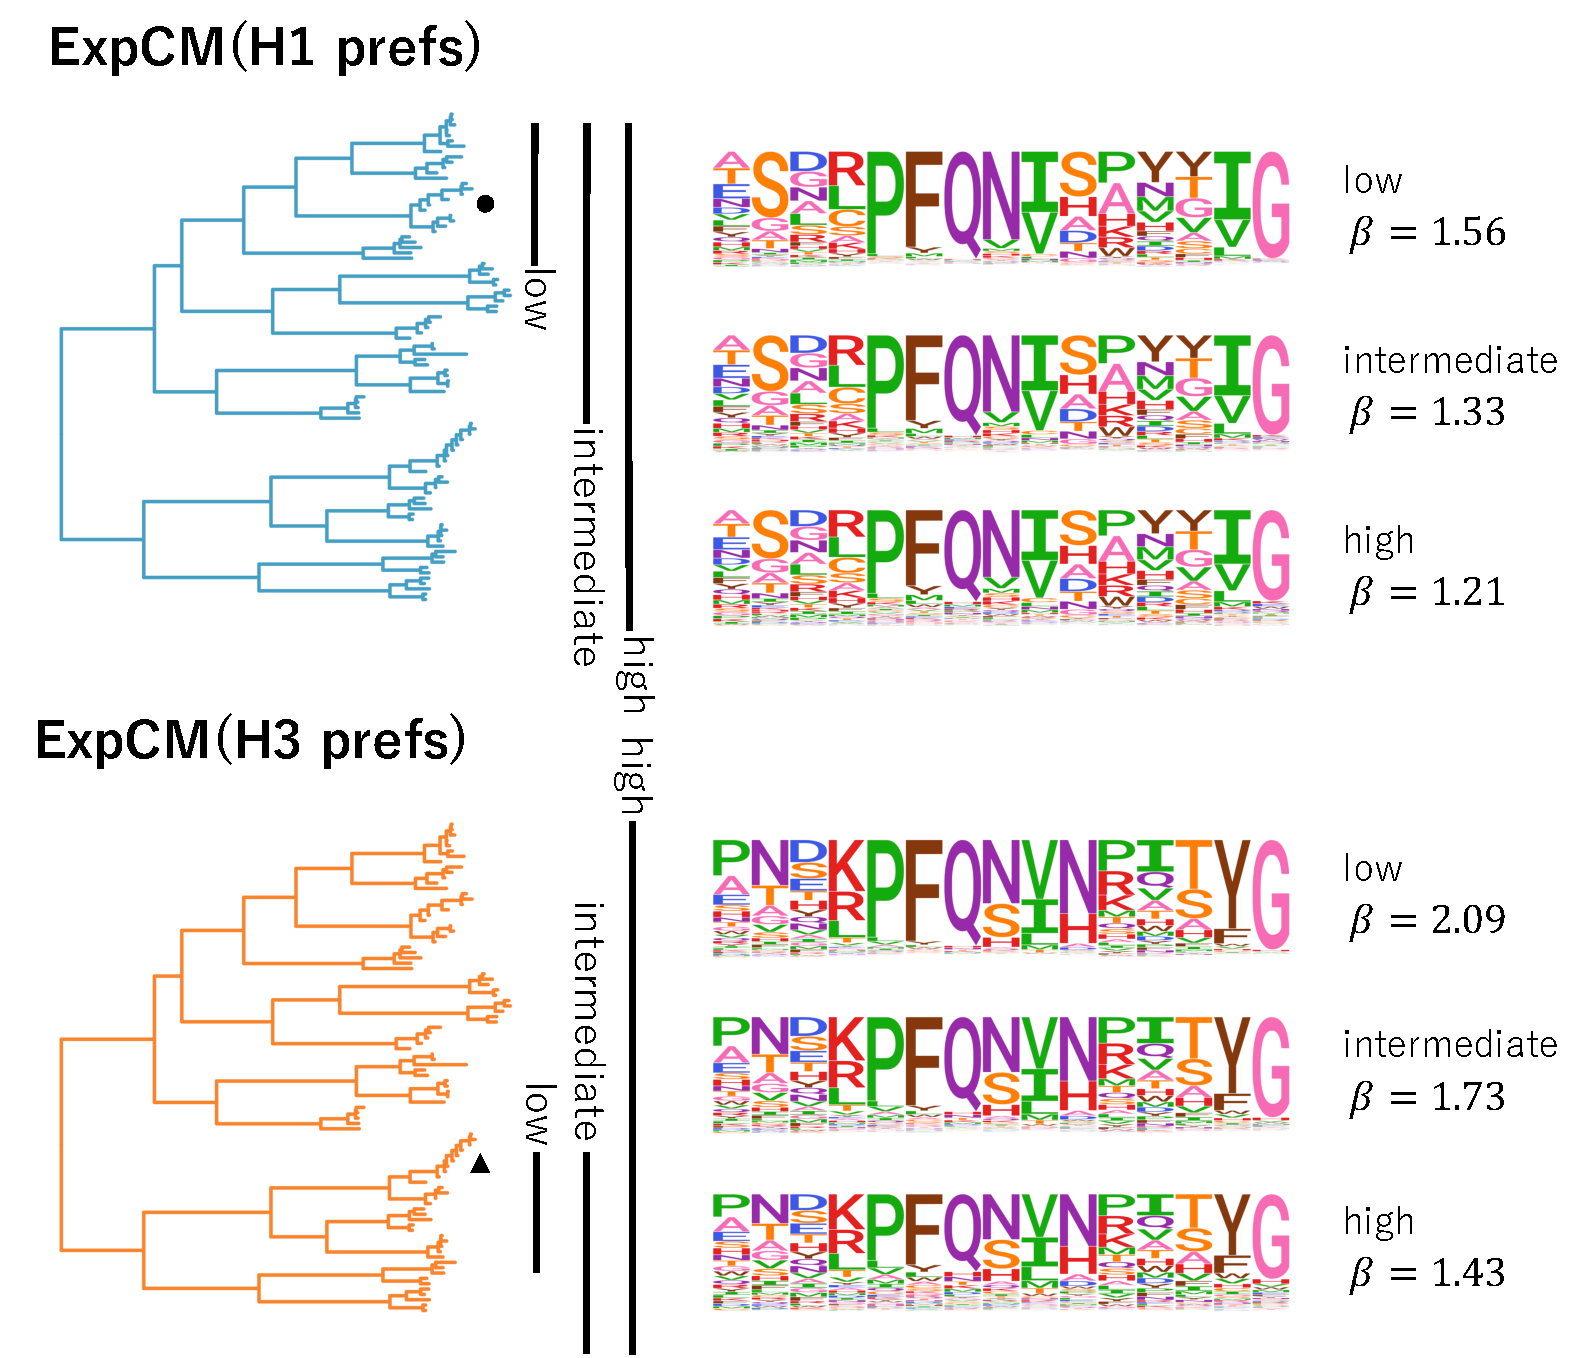
\includegraphics[width=0.75\textwidth]{figures/compete}}
\caption{\label{fig:compete}
\textbf{The congruency between natural selection and the deep mutational scanning measurements decreases with sequence divergence.} 
We fit an ExpCM informed by the H1 or H3 deep mutational scanning experiments to trees spanning sequences with low, intermediate, and high divergence from the sequence used in the experiment. 
The ExpCM stringency parameter ($\beta$) is a measure of the congruency between natural selection and the experimental measurements. 
Larger values of $\beta$ indicate that natural selection prefers the same amino acids as the experiments but with greater stringency. 
As divergence increases between the HA used in the experiment and the other sequences in the tree, the $\beta$ value decreases and the preference sets ``flatten."
Therefore, the preferences measured in each experiment are progressively less congruent with those of the HA sequences on the tree as we include increasingly diverged sequences. 
}
\end{figure}

The fact that an ExpCM has the greatest effect on branches close to the sequence used in the experiment can be rationalized in terms of existing knowledge about how epistasis shifts protein amino-acid preferences during evolution~\citep{pollock2012amino, shah2015contingency, doud2015site, haddox2017mapping, risso2014mutational}.
In reality, sites in proteins do not have completely conserved site-specific amino-acid preferences. 
Rather, the effect of a mutation at one site in a protein can depend on the amino-acid identity of other sites in the protein~\citep{starr2018pervasive, pollock2012amino, shah2015contingency, bazykin2015changing}. 
The deep mutational scanning experiments that inform our ExpCM's were performed in the context of a single HA genetic background, and so do not account for how such epistatic interactions can cause amino-acid preferences to shift as substitutions accumulate. 
Therefore, it makes sense that an ExpCM would most accurately describe the evolution of sequences closely related to the one used in the experiment.
 
We can clearly observe how shifting amino-acid preferences degrade the accuracy of the ExpCM by fitting them to trees containing increasingly diverged sequences.
Specifically, for H1 and H3 HAs, we created three phylogenetic trees: a ``low'' divergence tree that contains only sequences with $\ge 59\%$ amino-acid identity to the HA used in the experiment, an ``intermediate'' divergence tree that contains sequences with $\ge 46\%$ amino-acid identity to the HA in the experiment, and a ``high'' divergence tree that contains all the HAs (which have as little as 38\% identity to the HA in the experiment).
\ref{fig:compete} shows the subtrees containing each of these sets of HA sequences.
For each subtree, we examined the congruence between site-specific natural selection and the amino-acid preferences measured in the deep mutational scanning experiment. 
We used the ExpCM stringency parameter $\beta$ to measure this congruency~(\ref{eq:Frxy}). 
In essence, $\beta$ rescales the deep mutational scanning measurements~(\ref{fig:compete}). 
Larger values of $\beta$ indicate that natural selection prefers the same amino acids as the experiments but with a greater stringency, indicating a strong congruence between natural selection and the experimental preferences. 

\ref{fig:compete} shows that as the divergence from the sequence used in the deep mutational scan increases, the value of $\beta$ decreases. 
This inverse relationship between $\beta$ and overall divergence is seen for the ExpCM's informed by both the H1 and H3 experiments.
Specifically, as the $\beta$ value decreases, the preferences ``flatten" and draw less information from the experiment. 
At the most extreme, $\beta = 0$, the preferences would be perfectly uniform and look identical to the GY94 preferences in \ref{fig:empirical_trees}.
In reality, $\beta$ never reaches a value this low, indicating the deep mutational scanning experiments remain somewhat informative about the real purifying selection across the entire swath of HAs. 
However, the flattening with increasing sequence divergence arises because the amino-acid preferences are increasingly less accurate as we move away from the experimental sequence on the tree.
As shown in \ref{fig:simulations}, the ability of models with site-specific stationary states to extend branch lengths requires these stationary states to be accurate.
This fact also helps rationalize why the ExpCM defined by the average of the H1 and H3 experiments, representing the ``average" constraint on HA, does better across the whole tree (\ref{fig:empirical_trees}). 
 
The fact that amino-acid preferences shift as proteins evolve leaves us with an inherent tension: models with site-specific stationary states only become important for accurate branch-length estimation as sequences become increasingly diverged, but this same divergence degrades the accuracy of extrapolating the amino-acid preferences from any given experiment across the phylogenetic tree.
More importantly, the fact that amino-acid preferences shift over time means that there will not be any model with a single set of site-specific stationary states that accurately describes a phylogenetic tree that covers a wide span of sequences.

\subsection*{Models with stationary states estimated from natural sequences give similar results to ExpCM's}

\begin{figure}
\centerline{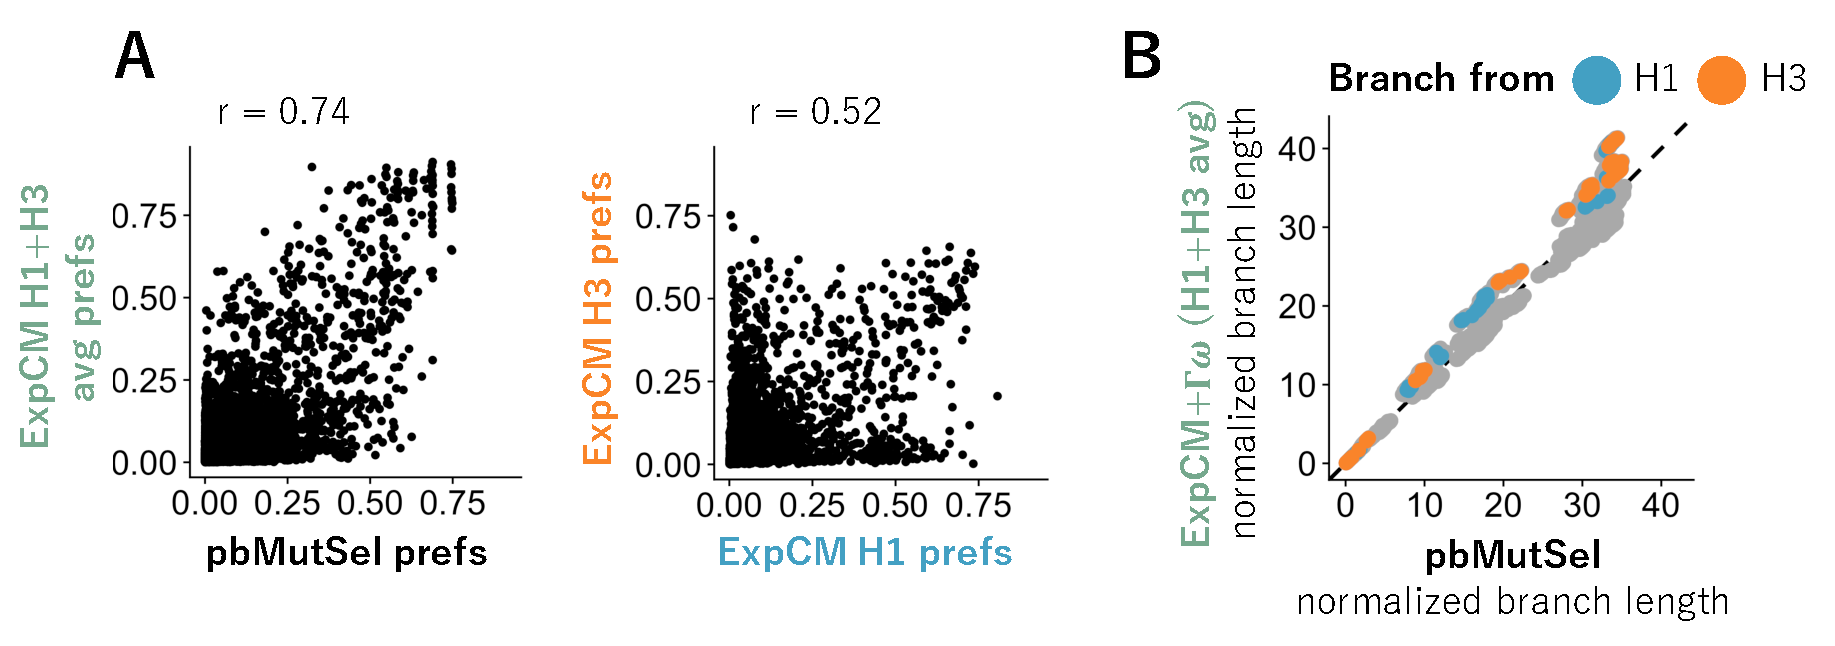
\includegraphics[width=0.99\textwidth]{figures/phylobayes.pdf}}
\caption{\label{fig:phylobayes}
\textbf{Models inferred from natural sequences have similar stationary states to models defined by experimental preferences and estimate similar branch lengths.}
(A) We fit an ExpCM(H1+H3 avg)+$\Gamma\omega$ and a pbMutSel to the tree in \ref{fig:empirical_trees}. 
The pbMutSel amino-acid preferences are inferred from the natural sequences while the ExpCM amino-acid preferences are experimentally measured and then rescaled using the stringency parameter in \ref{tab:empirical_data}. 
The pbMutSel preferences are more correlated with the average of the H1 and H3 deep mutational scanning preference sets than the individual experiments are to each other (Pearson's r: 0.74 vs. 0.52). 
(B) The pbMutSel and the ExpCM(H1+H3 avg)+$\Gamma\omega$ estimated similar branch lengths. 
To aid direct comparison between the models, we normalized the branch lengths by the length between and early and late seasonal human H1 sequence. 
}
\end{figure}

The previous sections used ExpCM's, which are mutation-selection models that use site-specific amino-acid preferences that have been measured by experiments. 
However, other implementations of mutation-selection models allow their stationary states to be inferred directly from the natural sequence data. 
These models are generally implemented in a Bayesian framework, which avoids the overfitting problems associated with trying to make maximum-likelihood estimates of the thousands of parameters describing site-specific stationary states.
The model most comparable to our ExpCM's is the codon mutation-selection model implemented in \texttt{phylobayes}, which we will refer to as pbMutSel~\citep{rodrigue2014site}. 
The pbMutSel model is mathematically very similar to the ExpCM's except the amino-acid preferences are modeled using Dirichlet processes rather than derived from experiments. 
Like ExpCM's, pbMutSel models still assume a single set of site-specific amino-acid preferences for the entire tree.

Comparing ExpCM's and pbMutSel models can therefore help identify the ultimate limits of mutation-selection models where each site has a single time-homogeneous stationary state across the entire tree. 
If the limits of the ExpCM's reflected in \ref{fig:empirical_trees} are simply because the deep mutational scanning experiments do not accurately measure the ``true" amino-acid preferences of HA across the tree, then we would expect the pbMutSel models (which derive their stationary states from the entire tree) to perform better.
On the other hand, if the major limitation is simply that there is not any single set of time-homogenous amino-acid preferences that describe HA evolution over the entire tree, then we would expect pbMutSel and ExpCM models to perform similarly.

The ExpCM that estimates the longest branches is the one that uses the average of the H1 and H3 deep mutational scanning measurements with $\Gamma\omega$ rate variation~(\ref{fig:empirical_trees}).  
We therefore compared this ExpCM with a pbMutSel model given the tree in \ref{fig:empirical_trees}. 
First, \ref{fig:phylobayes}A shows that the stationary state inferred by pbMutSel is similar to the average of the H1 and H3 preferences measured by deep mutational scanning. 
The site-specific amino-acid preferences estimated by pbMutSel are more correlated with the average amino-acid preferences from the H1 and H3 experiments than the individual deep mutational scanning experiments are to each other. 
This strong correlation between the pbMutSel and the average deep mutational scanning preference set indicates that, when averaged, the experimental preferences are able to capture the global site-specific functional constraint fairly well. 

Second, the results in \ref{fig:phylobayes}B show that the ExpCM+$\Gamma\omega$(H1+H3 avg prefs) and the pbMutSel model also estimated similar branch lengths on the HA tree in \ref{fig:empirical_trees}. 
While overall the two models estimated similar lengths, the tension between local and global accuracy of the amino-acid preferences is still apparent in these results. 
All the long branches from either the H1 or H3 sequences used in the experiments were estimated to be slightly longer by the ExpCM+$\Gamma\omega$, while many other branches were estimated to be slightly longer by the pbMutSel model. 
The relatively longer branches from the experimental sequences when using the ExpCM+$\Gamma\omega$ suggests that the ``global" stationary state inferred by \texttt{phylobayes} is not as accurate as the deep mutational scanning preferences for sequences close to the experimental sequences. 
However, at sequences distant from those used in the experiments, the ``global'' preferences estimated by the pbMutSel model appear to be slightly better than the average of the experimental values.
Therefore, while the site-specific pbMutSel models inferred by \texttt{phylobayes} are probably more accurate for sequences distant from the H1 and H3 in the experiments, they do not avoid the tension between the importance of a site-specific stationary state for long branch estimation and shifting preferences. 

\section*{Discussion}

Here, we tested the effect of models with site-specific stationary states on branch length estimation for the phylogenetic tree of highly diverged influenza HA sequences. 
We used site-specific stationary state models called ExpCM's, which are defined by amino-acid preferences measured by deep mutational scanning. 
We found that the ExpCM's estimated longer branches and did so independently from substitution rate variation via $\Gamma\omega$. 
We also found that the ExpCM's estimated branch lengths of a similar length to models which infer the stationary state from the natural sequences in a Bayesian framework.  

These results underscore the importance of modeling site-specific amino-acid preferences when estimating long branchs. 
As the simulations \ref{fig:simulations} show, models with uniform stationary states will always underestimate the lengths of branches which have evolved under site-specific constraints. 
The results with the influenza HA sequences shows that models with site-specific stationary states estimate longer branches when the stationary state is accurate. 
However, it is also clear that the accuracy of the ExpCM's stationary state degrades as the tree becomes more diverged from the HA used in the deep mutational scan. 
The desired effect of estimating long, accurate branches can only be achieved when the stationary state is accurate across the entire tree. 

However, it is clear from our results that a major limitation of site-independent, time-homogenous models is their inability to capture epistatic interactions. 
The site-specific amino-acid preferences of a protein shift across time and models with a single stationary state across the entire tree cannot capture these dynamics. 
The ExpCM's defined by preferences measured in one of two highly diverged HA's had the largest effect on branches near the HA from the experiment. 
The local effect of the ExpCM's defined by a single preference set indicate that different parts of the tree have different stationary states. 
This point is underscored by the comparison of the ExpCM defined by the average preference set and the pbMutSel model, which infers the stationary state from the natural sequences. 
Even though the stationary state of the pbMutSel model is more representative of the global stationary state, the ExpCM with average preferences has a larger effect on the branches from the H1 and H3 sequences. 
Therefore, while it is clear that modeling site-specific amino-acid preferences is important, neither one of these models is able to capture how these preferences shift over time.

Clearly, the site-independence and time-homogeneity assumptions of the ExpCM and pbMutSel models inhibit their ability to accurately describe the effect of epistasis.
In order to fully address the bias towards underestimation of divergence times by phylogenetic models, these models need to be able to accommodate how site-specific amino-acid preferences shift over time. 
One way to achieve this goal would be to void the site-independence assumption and create a model which explicitly describes the interactions between sites in a protein. 
However, while even modeling simple pairwise interactions would be a daunting task, epistasis could have higher order interactions which be extremely difficult to model. 
Another strategy would be to allow the stationary state to shift over lineages in the tree. 
Such a model might be still be site-independent but, by breaking the time-homogeneity assumption, would capture some effect of the shifting preferences. 
Models which account for epistasis would be inherently more complex but it clear from our results that it is important to capture how preferences shift over time to accurately estimate long branch lengths.

\section*{Materials and Methods}

\subsection*{Models}

\subsubsection*{GY94}

The GY94 model is defined as the M0 in \cite{yang2000codon}. 
$P_{xy}$ is the substitution rate from codon $x$ to codon $y$ and is defined by

\begin{equation}
\label{eq:GY94}
P_{xy} = 
\begin{cases}
  0 & \mbox{if $x$ and $y$ differ by more than one nucleotide,}\\
  \mu \omega \Phi_{y} & \mbox{if $x$ is converted to $y$ by a single-nucleotide transversion,} \\
  \kappa \mu \omega \Phi_{y} & \mbox{if $x$ is converted to $y$ by a single-nucleotide transition,} \\
  -\sum\limits_{z \ne x} P_{xz} & \mbox{if $x = y$.}
  \end{cases}
\end{equation}
where $\kappa$ is the transition-transversion ratio, $\Phi_y$ is the equilibrium frequency of
codon $y$, $\omega$ is the gene-wide rate of non-synonymous change, and $\mu$ is the substitution rate.
The stationary state of a GY94 model is defined as 
\begin{equation}
\label{eq:px}
p_{x} = \Phi_x
\end{equation}

\subsubsection*{Experimentally Informed Codon Model (ExpCM)}

In an ExpCM, the rate of substitution $P_{r,xy}$ of site $r$ from codon $x$ to $y$ is written in mutation-selection form~\citep{halpern1998evolutionary,mccandlish2014modeling,spielman2015relationship} as
\begin{equation}
\label{eq:ExpCM}
P_{r,xy} = Q_{xy} \times F_{r,xy}
\end{equation}
where $Q_{xy}$ is proportional to the rate of mutation from $x$ to $y$, and $F_{r,xy}$ is proportional to the probability that this mutation fixes.
The rate of mutation $Q_{xy}$ is assumed to be uniform across sites, and takes an HKY85-like~\citep{hasegawa1985dating} form.

The deep mutational scanning amino-acid preferences are incorporated into the ExpCM via the $F_{r,xy}$ terms.
The experiments measure the preference $\pi_{r,a}$ of every site $r$ for every amino-acid $a$.
The $F_{r,xy}$ terms are defined in terms of these experimentally measured amino-acid preferences as
\begin{equation}
\label{eq:Frxy}
F_{r,xy} = 
\begin{cases}
   1 & \mbox{if $\mathcal{A}\left(x\right) = \mathcal{A}\left(y\right)$} \\
   \omega \times \frac{\ln\left[\left(\pi_{r,\mathcal{A}\left(y\right)} / \pi_{r,\mathcal{A}\left(x\right)}\right)^{\beta}\right]}{1 - \left(\pi_{r,\mathcal{A}\left(x\right)} / \pi_{r,\mathcal{A}\left(y\right)}\right)^{\beta}} & \mbox{if $\mathcal{A}\left(x\right) \ne \mathcal{A}\left(y\right)$}
   \end{cases}
\end{equation}
where $\mathcal{A}\left(x\right)$ is the amino-acid encoded by codon $x$, $\beta$ is the stringency parameter, and $\omega$ is the relative rate of nonsynonymous to synonymous substitutions after accounting for the amino-acid preferences.

The stationary state of an ExpCM is defined as 
\begin{equation}
\label{eq:prx}
p_{r,x} = \frac{\phi_{x_1}\phi_{x_2}\phi_{x_3}\left(\pi_{r,A\left(x\right)}\right)^\beta}{\sum_z \phi_{z_1}\phi_{z_2}\phi_{z_3}\left(\pi_{r,A\left(z\right)}\right)^\beta}
\end{equation}
where $\phi_{x_1}$, $\phi_{x_2}$, and $\phi_{x_3}$ are the nucleotides at position 1, 2, and 3 of codon $x$. 

The preferences $\pi_{r,a}$ are \emph{not} free parameters since they are determined by an experiment independent of the sequence alignment being analyzed.
The ExpCM is described in detail in~\citet{hilton2017phydms}. 

\subsubsection*{GY94 with $\omega_r$.}

We defined a site-specific model with the GY94 stationary state by multiplying the $\omega$ in \ref{eq:GY94} with a site-specific $\omega_r$ value calculated from an ExpCM (\ref{eq:ExpCM}). 
Specifically, following \citet{spielman2015relationship}, 
\begin{equation}
\label{eq:w_r}
\omega_{r} = \frac{\sum_{x} \sum_{y \in N_x} {p_{r,x} \times \frac{P_{r,xy}}{\omega}}}{\sum_{x} \sum_{y \in N_x} {p_{r,x} \times Q_{xy}}}
\end{equation}
where $p_{r,x}$ is the stationary state of the ExpCM at site $r$ and codon $x$, $P_{r,xy}$ is the substitution rate from codon $x$ to codon $y$ at site $r$, $Q_{xy}$ is the mutation rate from codon $x$ to codon $y$, $\omega$ is the relative nonsynonymous substitution rate from the ExpCM and $N_x$ is the set of codons that are nonsynonymous to codon $x$ and differ from codon $x$ by only one nucleotide. 

\subsection*{$\Gamma\omega$ rate variation.}

The GY94+$\Gamma\omega$ is defined as M5 in \citet{yang2000codon} and the ExpCM+$\Gamma\omega$ follows the same logic. 
Briefly, $\omega$ is drawn from a $\Gamma$ distribution discretized into $K=4$ bins. 
Each bin is equally weighted and $\omega$ takes on the mean value of the bin. 

\subsection*{Deep mutational scanning amino-acid preferences.}
We used amino-acid preferences measured in the deep mutational scans of an H1 HA~\citep{doud2016accurate} and an H3 HA~\citep{lee2018deep} to define the ExpCM $\pi_{r, A\left(x\right)}$ parameters~(\ref{eq:Frxy}). 
We only considered sites which are homologous between H1 HA and H3 HA. 
These homologous sites, and their mapping between the H1 reference strain A/Wilson Smith/1933 and the H3 reference strain a A/Perth/2009, are described in \ref{suppfile:WSN_Perth_map}. 
The resulting preference sets, including the average between the H1 and H3 preferences, are found in \ref{suppfile:H1_prefs}, \ref{suppfile:H3_prefs}, and \ref{suppfile:avg_prefs}.

\subsection*{Influenza virus hemagglutinin (HA) sequences and tree topology.}

We downloaded all full-length, coding sequences for 14 of the 18 HA subtypes, excluding the rare subtypes 12, 15, 17, and 18. 
We filtered and aligned the sequences using \texttt{phydms\_prepalignment}~\citep{hilton2017phydms}. 
Specifically, we used \texttt{phydms\_prepalignment} with the flag \texttt{--minidentity 0.3} to remove sequences with ambiguous nucleotides, premature stops, or frameshift mutations as well as redundant sequences.  
We also removed any codon sites which are not shared between the H1 HA and H3 HA used in the deep mutational scanning experiments. 
We subsampled the remaining sequences to five sequences per subtype with $\le 1$ sequence per year per subtype. 
We also included a small number of representative sequences from the major human and equine influenza lineages, described in \ref{suppfile:required_seqs}. 
The resulting alignment contains 87 sequences and is found in \ref{suppfile:alignment_high}. 

We created four subalignments with ``low" and ``intermediate" divergence from either the H1 or the H3 deep mutational scanning reference sequence. 
The ``low divergence" alignments had   $\ge 59\%$ amino-acid identity from the reference sequence and the ``intermediate divergence" alignments had $\ge 46\%$ identity from the reference sequence.
The resulting alignments are found in \ref{suppfile:alignment_lowH1}, \ref{suppfile:alignment_lowH3}, \ref{suppfile:alignment_intermediateH1}, and \ref{suppfile:alignment_intermediateH3}.  

We inferred the tree topology of each alignment using \texttt{RAxML}~\citep{stamatakis2006raxml} and the GTRCAT model. 
We estimated the branch lengths of this fixed topology using the ExpCM and GY94 models with \texttt{phydms\_comprehensive}~\citep{hilton2017phydms}. 

\subsection*{Asymptotic sequence divergence.}

We defined ExpCM and GY94 models using parameter values fit to the ``low divergence from H1" tree~(\ref{fig:empirical_trees}, \ref{suppfile:alignment_lowH1}). 
Specifically, we defined the GY94 model using the parameter values in~\ref{suppfile:hybrid_lowH1_GY94}, the GY94+$\Gamma\omega$ using the parameter values in~\ref{suppfile:hybrid_lowH1_GY94+Gr} and the ExpCM using the parameter values in~\ref{suppfile:hybrid_lowH1_ExpCMdoud} and the H1 amino-acid preferences from~\citet{doud2016accurate} in~\ref{suppfile:H1_prefs}. 

For each model, we calculated the expected sequence divergence given branch length $t$ by 
\begin{equation}
\label{eq:f}
\sum_a \sum_{x \in a} p_{r,x} \sum_{y \in a} [M_{r}\left(t\right)]_{xy}
\end{equation}
where $a$ is all amino acids, $p_{r,x}$ is the stationary state of the model at site $r$ and codon $x$, and $[M_{r}\left(t\right)]_{xy}$ is the transition rate from codon $x$ to codon $y$ at site $r$ given time $t$. 

\subsection*{Simulations}

We simulated sequences using \texttt{pyvolve}~\citep{spielman2015pyvolve} along the tree for the full alignment (\ref{fig:empirical_trees}, \ref{suppfile:alignment_high}) using an ExpCM defined by parameters fit to the ``low divergence from H1 tree" (\ref{suppfile:alignment_lowH1}). 
Specifically, we defined the ExpCM using the parameter values in \ref{suppfile:hybrid_lowH1_ExpCMdoud} and the H1 amino-acid preferences from \citet{doud2016accurate} in \ref{suppfile:H1_prefs}. 
We performed 10 replicate simulations and estimated the branch lengths for each replicate using \texttt{phydms\_comprehensive}~\citep{hilton2017phydms}. 

\subsection*{pbMutSel inference with \texttt{phylobayes}.}

We inferred a pbMutSel model for the full tree (\ref{fig:empirical_trees}, \ref{suppfile:alignment_high}). 
We ran one chain for 5000 steps, saved every sample, and discarded the first 500 samples as a burnin. 
We normalized the branch lengths on the pbMutSel consensus tree and the ExpCM(H1+H3 avg)+$\Gamma\omega$ by dividing each branch by the length from A/South Carolina/1/1918 and A/Solomon Islands/3/2006. 
These two H1 sequences are early and late representatives of the longest known human influenza lineage. 

\subsection*{Code and analysis.}
All code used is available at \url{https://github.com/jbloomlab/divergence_timing_manuscript}. 
For the main analysis, we used \texttt{phydms}~\citep{hilton2017phydms} version 2.2.dev2 (available at \url{github.com/jbloomlab/phydms}) to filter sequences and estimate branch lengths, \texttt{pyvolve}~\citep{spielman2015pyvolve} version 0.8.7 (available at \url{https://github.com/sjspielman/pyvolve}) to simulate the sequences and \texttt{phylobayes}~\citep{rodrigue2014site} version 1.8 (available at \url{https://github.com/bayesiancook/pbmpi}) to infer the pbMutSel model. We also used \texttt{ggplot2}~\citep{wickham2016ggplot2}, \texttt{ggtree}~\citep{yu2017ggtree}, and \texttt{ggseqlogo}~\citep{wagih2017ggseqlogo} for visualization.



\newpage
\section*{Supplemental Information}

\begin{suppfig}[H]
\centerline{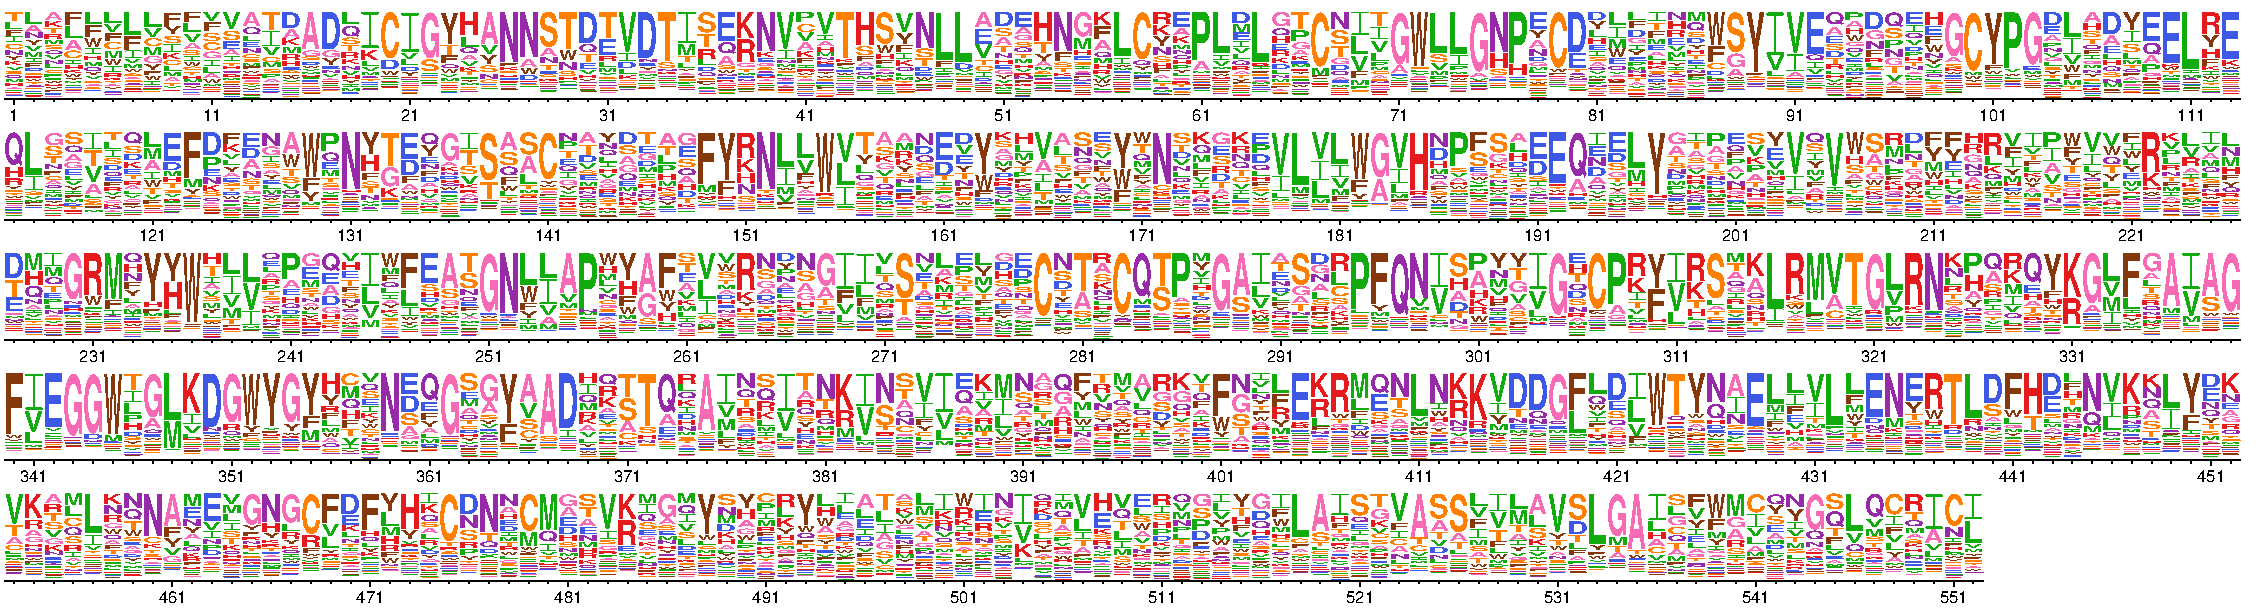
\includegraphics[width=\textwidth]{figures/prefs_doud}}
\caption{\label{suppfig:prefs_doud}
\textbf{H1 HA amino-acid preferences measured by deep mutational scanning.}
Each column represents a site in the protein and the height of each letter is proportional to the preference for the amino acid as measured by~\citet{doud2016accurate}. 
Here the preferences are rescaled by the ExpCM stringency parameter in \ref{tab:empirical_data} ($\beta=1.12$). 
We only considered homologous sites between H1 and H3. 
The conversion between the numbering scheme in this figure and sequential numbering of the H1 HA reference sequence A/Wilson Smith/1933 is found in \ref{suppfile:WSN_Perth_map}. 
}
\end{suppfig}

\begin{suppfig}[H]
\centerline{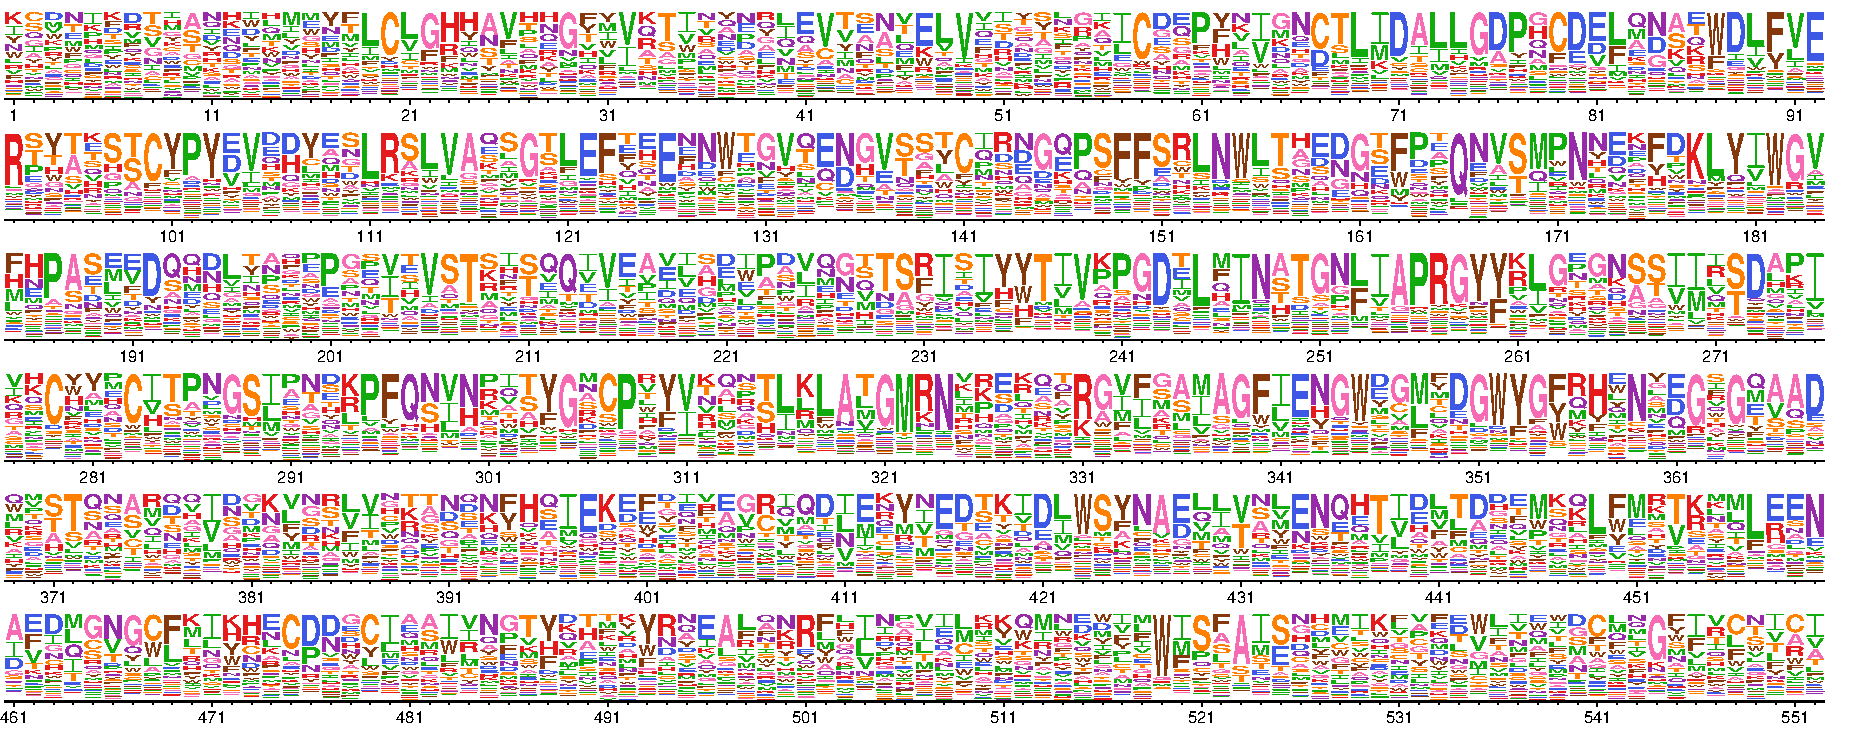
\includegraphics[width=\textwidth]{figures/prefs_lee}}
\caption{\label{suppfig:prefs_lee}
\textbf{H3 HA amino-acid preferences measured by deep mutational scanning.}
Each column represents a site in the protein and the height of each letter is proportional to the preference for the amino acid as measured by~\citet{lee2018deep}. 
Here the preferences are rescaled by the ExpCM stringency parameter in \ref{tab:empirical_data} ($\beta=1.28$). 
We only considered homologous sites between H1 and H3. 
The conversion between the numbering scheme in this figure and sequential numbering of the H3 HA reference sequence A/Perth/2009 is found in \ref{suppfile:WSN_Perth_map}. 
 }
\end{suppfig}

\begin{suppfig}[H]
\centerline{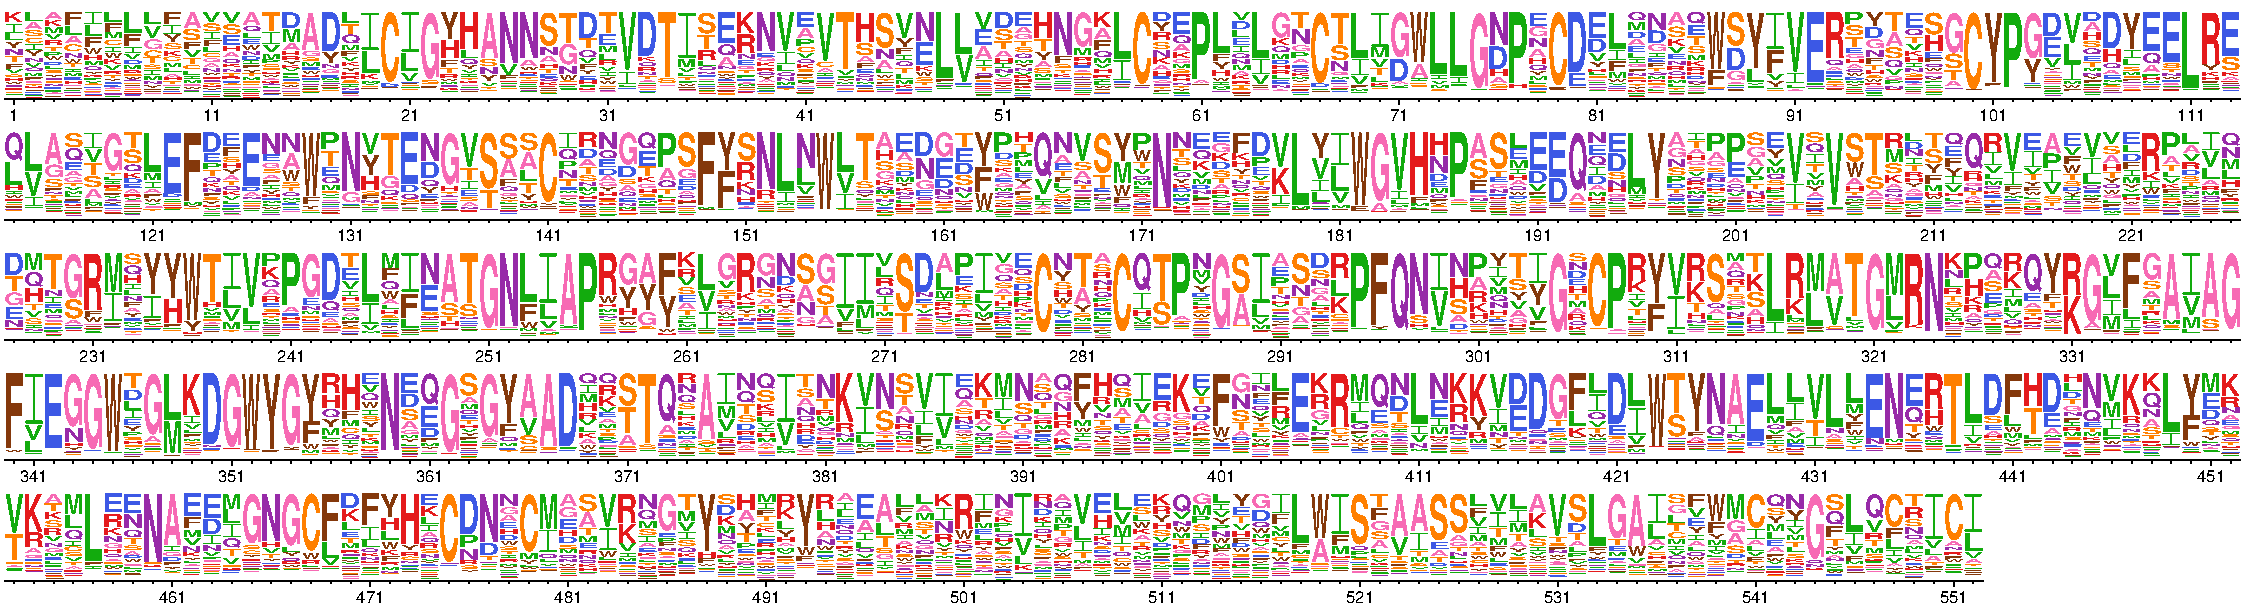
\includegraphics[width=\textwidth]{figures/prefs_average}}
\caption{\label{suppfig:prefs_average}
\textbf{Average of H1 HA  and H3 HA amino-acid preferences measured by deep mutational scanning.}
Each column represents a site in the protein and the height of each letter is proportional to the average preference for the amino acid measured by~\citet{doud2016accurate} and~\citet{lee2018deep}. 
Here the preferences are rescaled by the ExpCM stringency parameter in \ref{tab:empirical_data} ($\beta=1.70$). 
We only considered homologous sites between H1 and H3. 
The conversion between the numbering scheme in this figure and sequential numbering of the H1 HA reference sequence A/Wilson Smith/1933 or H3 HA reference sequence A/Perth/2009 is found in \ref{suppfile:WSN_Perth_map}. 
}
\end{suppfig}

\begin{suppfig}[H]
\centerline{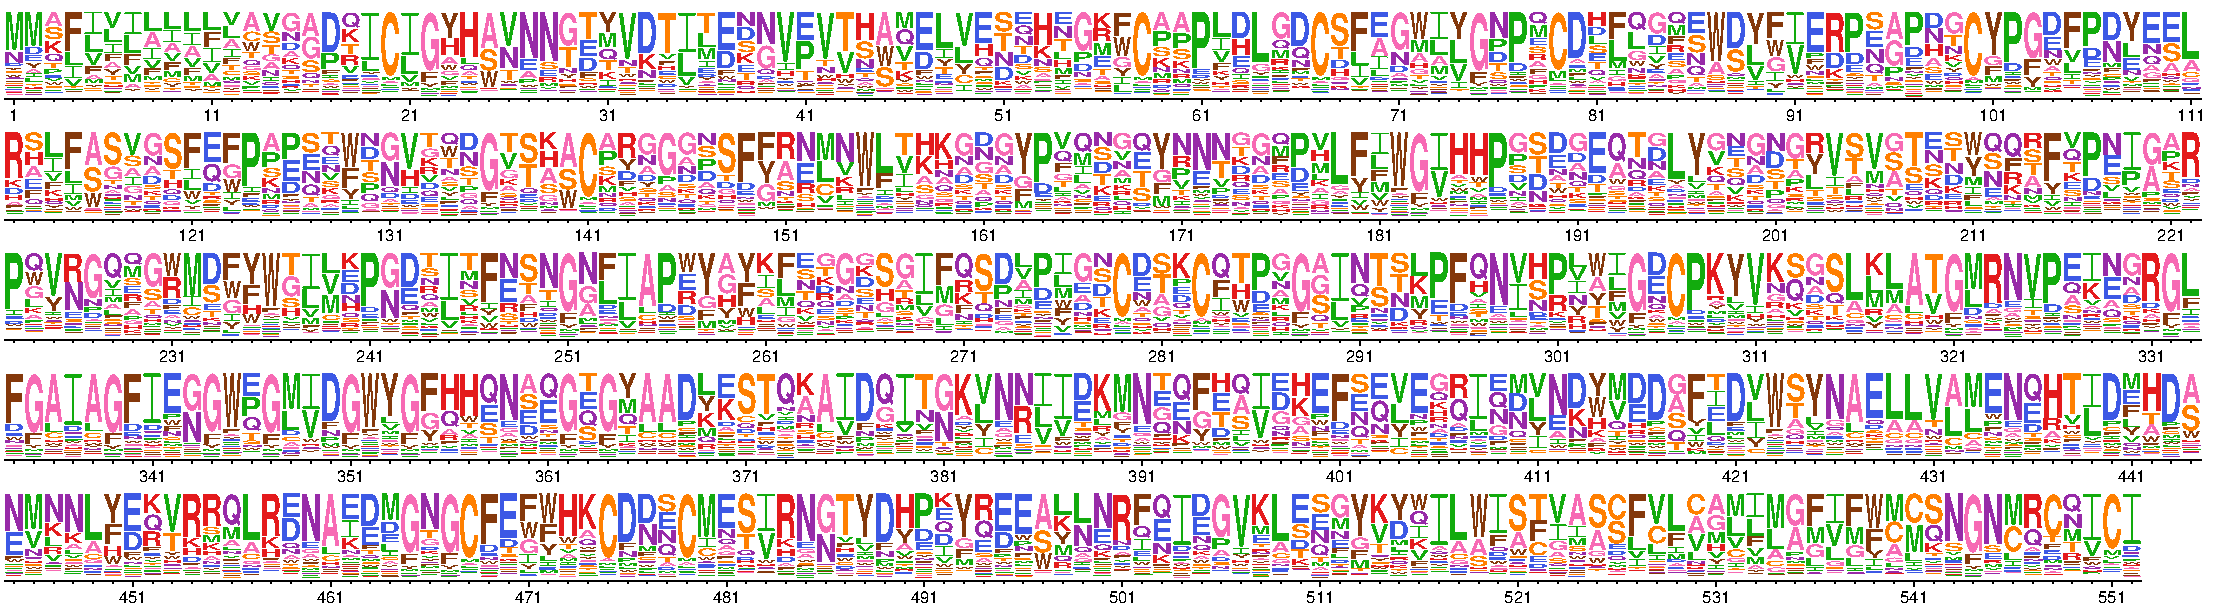
\includegraphics[width=\textwidth]{figures/prefs_mutSel}}
\caption{\label{suppfig:prefs_mutSel}
\textbf{Amino-acid preferences inferred by the pbMutSel model.}
Each column represents a site in the protein and the height of each letter is proportional to the preference for the amino acid inferred by pbMutSel~\citep{rodrigue2014site} using the tree in \ref{fig:empirical_trees}. 
We only considered homologous sites between H1 and H3. 
The conversion between the numbering scheme in this figure and sequential numbering of the H1 HA reference sequence A/Wilson Smith/1933 or H3 HA reference sequence A/Perth/2009 is found in \ref{suppfile:WSN_Perth_map}. 
}
\end{suppfig}

\begin{suppfig}[H]
\centerline{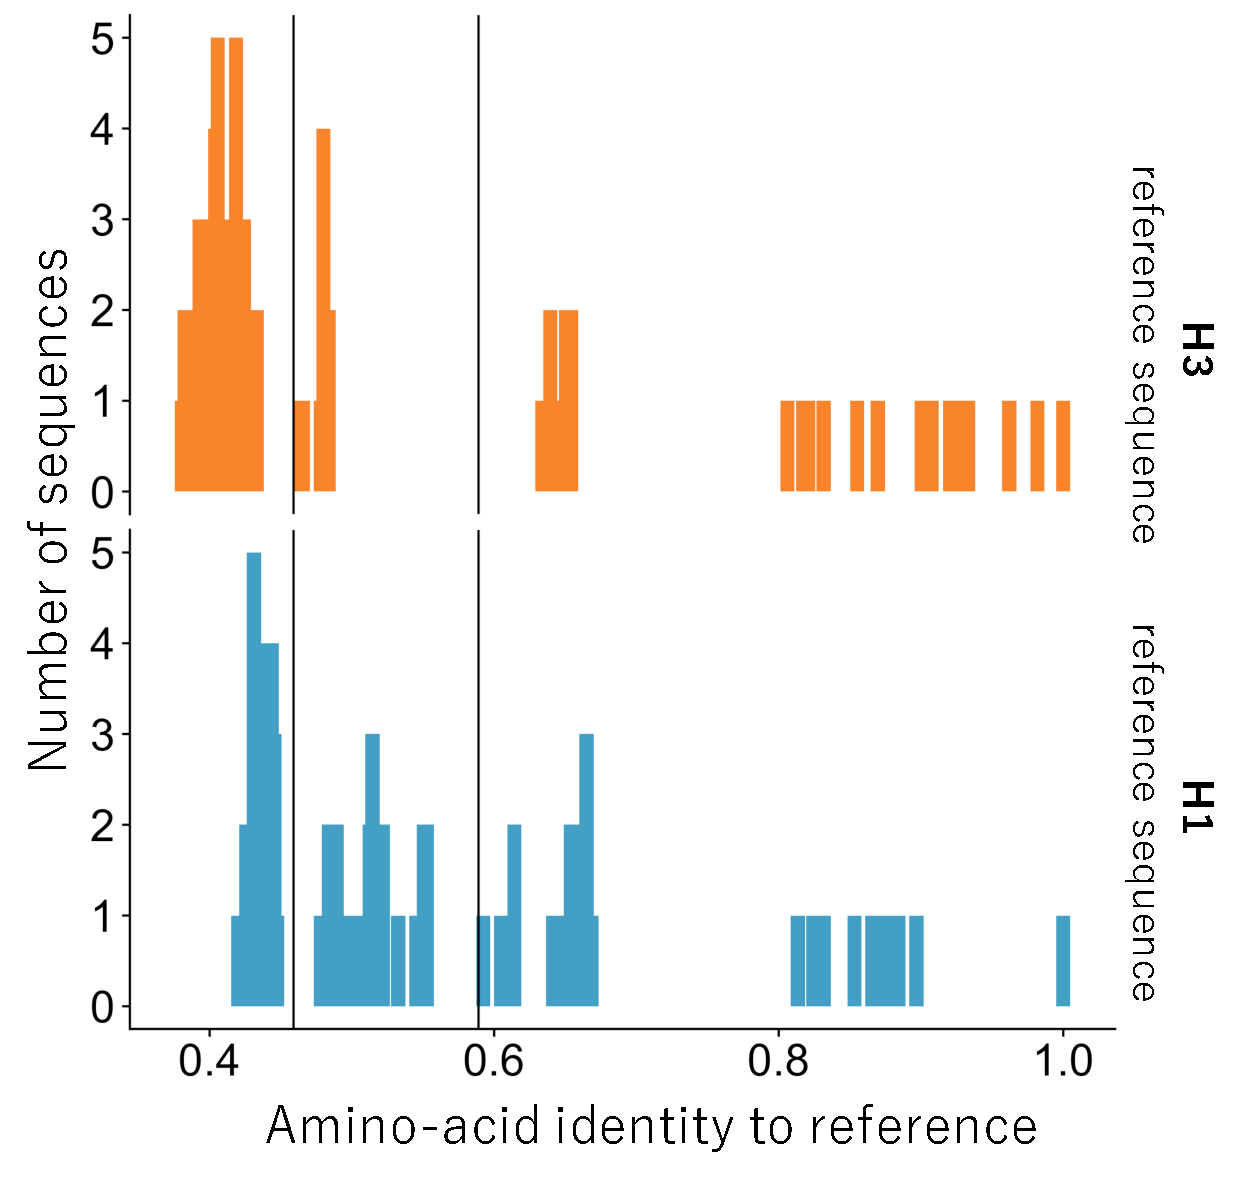
\includegraphics[width=0.50\textwidth]{figures/divergence_distances.pdf}}
\caption{\label{suppfig:subalignments}
\textbf{Overall divergence for the subtrees in \ref{fig:compete}.} 
We created two sub alignments from the alignment (\ref{suppfile:alignment_high}) used in \ref{fig:empirical_trees} for each deep mutational scanning reference HA. 
The ``low" alignments have $\ge59\%$ amino-acid identity to the reference sequence (\ref{suppfile:alignment_lowH1}, \ref{suppfile:alignment_lowH3}) and the ``intermediate" alignments have $\ge46\%$ amino-acid identity to the reference sequence (\ref{suppfile:alignment_intermediateH1}, \ref{suppfile:alignment_intermediateH3}).
}
\end{suppfig}

\begin{table}[t!]
\caption{\label{supptab:tree_lengths}
{\bf Total branch length for the trees in \ref{fig:empirical_trees}.}
The branch lengths are in average codon substitutions per site. 
} 
     \begin{tabular}{cccccccccc}
        \hline
         Model & no rate variation & {\shortstack{$\Gamma\omega$ rate\\ variation}} \\ \hline
         GY94 &53.05 & 72.28\\
         ExpCM (H1) & 57.32 & 81.31\\
         ExpCM (H3) & 57.77 & 78.98\\
         ExpCM(H1 + H3 avg) & 62.98 & 83.96 \\
      \end{tabular}
\end{table}

%%%

\begin{suppfile}
\caption{
\label{suppfile:WSN_Perth_map}
Map for homologous sites between H1 HA and H3 HA. 
This file provides a conversion between the numbering scheme we use in the paper, including all logoplots and the sites in \ref{fig:decay}, to sequential numbering in either the H1 HA reference sequence A/Wilson Smith/1933 or the H3 HA reference sequence A/Perth/2009. 
The sequential numbering for the HA strains starts with ``site 1" as the second codon (first non-methionine codon). 
}
\end{suppfile}

\begin{suppfile}
\caption{
\label{suppfile:H1_prefs}
Amino acid preferences measured by the deep mutational scanning of the H1 HA strain A/Wilson Smith/1933~\citep{doud2016accurate}. 
This file only contains measurements for the homologous sites between H1 HA and H3 HA. 
Conversion from this numbering scheme to sequential numbering in A/Wilson Smith/1933 is found in \ref{suppfile:WSN_Perth_map}. 
}
\end{suppfile}

\begin{suppfile}
\caption{
\label{suppfile:H3_prefs}
Amino acid preferences measured by the deep mutational scanning of the H3 HA strain A/Perth/2009~\citep{lee2018deep}. 
This file only contains measurements for the homologous sites between H1 HA and H3 HA. 
Conversion from this numbering scheme to sequential numbering in A/Perth/2009 is found in \ref{suppfile:WSN_Perth_map}. 
}
\end{suppfile}

\begin{suppfile}
\caption{
\label{suppfile:avg_prefs}
Average of the amino acid preferences measured by the deep mutational scanning of the H1 HA strain A/Wilson Smith/1933~\citep{doud2016accurate} and the H3 HA strain A/Perth/2009~\citep{lee2018deep}. 
This file only contains measurements for the homologous sites between H1 HA and H3 HA. 
Conversion from this numbering scheme to sequential numbering in A/Wilson Smith/1933 or A/Perth/2009 is found in \ref{suppfile:WSN_Perth_map}. }
\end{suppfile}

\begin{suppfile}
\caption{
\label{suppfile:required_seqs}
This file contains the representative sequences of major human equine influenza lineages added to the alignment in \ref{suppfile:alignment_high}. 
}
\end{suppfile}

\begin{suppfile}
\caption{
\label{suppfile:alignment_high}
The HA sequences used for the full HA tree in \ref{fig:empirical_trees}. 
We inferred the topology using \texttt{RAxML} and the GTRCAT model. 
}
\end{suppfile}

\begin{suppfile}
\caption{
\label{suppfile:alignment_lowH1}
The HA sequences using for the ``low divergence from H1" tree in \ref{fig:compete}. 
All sequences have $\ge 59\%$ amino-acid identity to the H1 reference sequence A/Wilson Smith/1933. 
We inferred the topology using \texttt{RAxML} and the GTRCAT model. 
}
\end{suppfile}

\begin{suppfile}
\caption{
\label{suppfile:alignment_lowH3}
The HA sequences using for the ``low divergence from H3" tree in \ref{fig:compete}. 
All sequences have $\ge 59\%$ amino-acid identity to the H3 reference sequence A/Perth/2009. 
We inferred the topology using \texttt{RAxML} and the GTRCAT model. 
}
\end{suppfile}

\begin{suppfile}
\caption{
\label{suppfile:alignment_intermediateH1}
The HA sequences using for the ``intermediate divergence from H1" tree in \ref{fig:compete}. 
All sequences have $\ge 46\%$ amino-acid identity to the H1 reference sequence A/Wilson Smith/1933. 
We inferred the topology using \texttt{RAxML} and the GTRCAT model. 
}
\end{suppfile}

\begin{suppfile}
\caption{
\label{suppfile:alignment_intermediateH3}
The HA sequences using for the ``intermediate divergence from H3" tree in \ref{fig:compete}. 
All sequences have $\ge 46\%$ amino-acid identity to the H3 reference sequence A/Perth/2009. 
We inferred the topology using \texttt{RAxML} and the GTRCAT model. 
}
\end{suppfile}

\begin{suppfile}
\caption{
\label{suppfile:hybrid_lowH1_GY94}
The GY94 model parameters fit to the ``low divergence from H1" tree (\ref{fig:compete}, \ref{suppfile:alignment_lowH1}). 
The model was fit using \texttt{phydms\_comprehensive}. 
}
\end{suppfile}

\begin{suppfile}
\caption{
\label{suppfile:hybrid_lowH1_GY94+Gr}
The GY94+$\Gamma\omega$ model parameters fit to the ``low divergence from H1" tree (\ref{fig:compete}, \ref{suppfile:alignment_lowH1}). 
The model was fit using \texttt{phydms\_comprehensive}. 
}
\end{suppfile}

\begin{suppfile}
\caption{
\label{suppfile:hybrid_lowH1_ExpCMdoud}
The ExpCM model parameters fit to the ``low divergence from H1" tree (\ref{fig:compete}, \ref{suppfile:alignment_lowH1}). 
The model was fit using \texttt{phydms\_comprehensive} and the H1 HA amino-acid preference set in \ref{suppfile:H1_prefs}. 
}
\end{suppfile}

\clearpage 
\bibliographystyle{mbe}
\bibliography{references.bib}



\end{document}